% $Header: /cvsroot/latex-beamer/latex-beamer/solutions/conference-talks/conference-ornate-20min.en.tex,v 1.7 2007/01/28 20:48:23 tantau Exp $

\documentclass{beamer}
\usepackage{verbatim}
\usepackage{mathtools}
\usepackage{multirow} 
\usepackage{amsmath}
\usepackage{tikz}

\usetikzlibrary{shapes.geometric,arrows}
\tikzstyle{rn} = [circle, text centered, very thick, draw=black, fill=blue!20]
\tikzstyle{rn_ig} = [circle, text centered, draw=black!40, fill=blue!10]
\tikzstyle{po} = [circle, text centered, very thick, draw=black, fill=red!20]
\tikzstyle{po_ig} = [circle, text centered, draw=black!40, fill=red!10]
\tikzstyle{pb} = [circle, text centered, very thick, draw=black, fill=yellow!20]
\tikzstyle{pb_ig} = [circle, text centered, draw=black!40, fill=yellow!10]
\tikzstyle{at} = [circle, text centered, very thick, draw=black, fill=green!30]
\tikzstyle{at_ig} = [circle, text centered, draw=black!40, fill=green!15]
\tikzstyle{bi} = [circle, text centered, very thick, draw=black, fill=cyan!20]
\tikzstyle{bi_ig} = [circle, text centered, draw=black!40, fill=cyan!10]
\tikzstyle{tl} = [circle, text centered, very thick, draw=black, fill=magenta!40]
\tikzstyle{tl_ig} = [circle, text centered, draw=black!40, fill=magenta!20]

\tikzstyle{ignuc} = [circle, text centered, draw=black!40, fill=white]

% This file is a solution template for:

% - Talk at a conference/colloquium.
% - Talk length is about 20min.
% - Style is ornate.



% Copyright 2004 by Till Tantau <tantau@users.sourceforge.net>.
%
% In principle, this file can be redistributed and/or modified under
% the terms of the GNU Public License, version 2.
%
% However, this file is supposed to be a template to be modified
% for your own needs. For this reason, if you use this file as a
% template and not specifically distribute it as part of a another
% package/program, I grant the extra permission to freely copy and
% modify this file as you see fit and even to delete this copyright
% notice.

%%%%%%%%%%%%%%%%%%%%%%%%%%%% THEME  %%%%%%%%%%%%%%%%%%%%%%%%%%%%%%%%%
 % \usetheme{AnnArbor}
  %\usetheme{Antibes}
  %\usetheme{Bergen}
  %\usetheme{Berkeley}
  %\usetheme{Berlin}
  %\usetheme{Boadilla}
  %\usetheme{boxes}
  %\usetheme{CambridgeUS}
  %\usetheme{Copenhagen}
  %\usetheme{Darmstadt}
  %\usetheme{default}
  %\usetheme{Dresden}
  \usetheme{Frankfurt}
  %\usetheme{Goettingen}
  %\usetheme{Hannover}
  %\usetheme{Ilmenau}
  %\usetheme{JuanLesPins}
  %\usetheme{Luebeck}
  %\usetheme{Madrid}
  %\usetheme{Malmoe}
  %\usetheme{Marburg}
  %\usetheme{Montpellier}
  %\usetheme{PaloAlto}
  %\usetheme{Pittsburgh}
  %\usetheme{Rochester}
  %\usetheme{Singapore}
  %\usetheme{Szeged}
  %\usetheme{Warsaw}

  %%%%%%%%%%%%%%%%%%%%%%%%%%%% COLOR THEME  %%%%%%%%%%%%%%%%%%%%%%%%%%%%%%%%%
  %\usecolortheme{albatross}
  %\usecolortheme{beetle}
  %\usecolortheme{beaver} %****
  %\usecolortheme{crane} %****
  %\usecolortheme{default} %****
  %\usecolortheme{dolphin} %****
  %\usecolortheme{dove} %****
  %\usecolortheme{fly}
  %\usecolortheme{lily}
\usecolortheme{orchid}
  %\usecolortheme{rose}
  %\usecolortheme{seagull}
  %\usecolortheme{seahorse}
  %\usecolortheme{sidebartab}
  %\usecolortheme{structure}
  %\usecolortheme{whale}
  %\usecolortheme{wolverine}

  %%%%%%%%%%%%%%%%%%%%%%%%%%%% OUTER THEME  %%%%%%%%%%%%%%%%%%%%%%%%%%%%%%%%%
  %\useoutertheme{default}
  %\useoutertheme{infolines}
  %\useoutertheme{miniframes}
  %\useoutertheme{shadow}
  %\useoutertheme{sidebar}
  %\useoutertheme{smoothbars}
  %\useoutertheme{smoothtree}
  %\useoutertheme{split}
  %\useoutertheme{tree}

  %%%%%%%%%%%%%%%%%%%%%%%%%%%% INNER THEME  %%%%%%%%%%%%%%%%%%%%%%%%%%%%%%%%%
  %\useinnertheme{circles}
  %\useinnertheme{default}
  %\useinnertheme{inmargin}
  %\useinnertheme{rectangles}
  %\useinnertheme{rounded}

  %%%%%%%%%%%%%%%%%%%%%%%%%%%%%%%%%%% color %%%%%%%%%%%%%%%%%%%%%%%%%%%%%%%%%

\usefonttheme{serif}

\definecolor{columbiablue0}{rgb}{ 0.8078431,0.9372549,1}
\definecolor{columbiablue1}{rgb}{0,.808,0}
\definecolor{columbiablue2}{rgb}{0.1764706,0.1647059,0.3843137}
\definecolor{columbiablue3}{rgb}{0,0.4,0.08}
\definecolor{columbiablue4}{rgb}{0.1921569,0.3058824,0.5137255}
\definecolor{columbiablue5}{rgb}{0.1,0.5215686,0.2}
\usecolortheme[named=columbiablue3]{structure}
\setbeamercolor{frametitle}{fg=columbiablue5,bg=white}
\usepackage{beamerthemesplit}

\usepackage[english]{babel}
% or whatever
\usepackage[latin1]{inputenc}
% or whatever
\usepackage{times}
\usepackage[T1]{fontenc}
% Or whatever. Note that the encoding and the font should match. If T1
% does not look nice, try deleting the line with the fontenc.

%\definecolor{UniBlue}{RGB}{83,121,170}
%\setbeamercolor{title}{fg=UniBlue}
%\setbeamercolor{frametitle}{fg=UniBlue}
%\setbeamercolor{structure}{fg=UniBlue}

%\setbeamertemplate{footline}{
%   \unilogo
%   \dsglogo
%   \begin{beamercolorbox}[ht=4ex,leftskip=1.4cm,rightskip=.3cm]{author in head/foot}
%    \usebeamercolor{UniBlue}
%    \hrule
%    \vspace{0.1cm}
%    \insertdate \hfill \inserttitle \newline
%    \insertshortauthor \ - \insertshortinstitute \hfill \insertframenumber
%   \end{beamercolorbox}
%   \vspace*{0.1cm}
%}
\newcommand{\nologo}{\setbeamertemplate{logo}{}}

\defbeamertemplate*{footline}{information lines theme without institution and slide numbers}
{
  \leavevmode%
  \unilogo
  \hbox{%
  \begin{beamercolorbox}[wd=.333333\paperwidth,ht=2.5ex,dp=1ex,center]{author in head/foot}%
    \usebeamerfont{author in head/foot}\insertshortauthor ~~(\insertshortinstitute)
  \end{beamercolorbox}%
  \begin{beamercolorbox}[wd=.333333\paperwidth,ht=2.5ex,dp=1ex,center]{title in head/foot}%
    \usebeamerfont{title in head/foot}\insertshorttitle
  \end{beamercolorbox}%
  \begin{beamercolorbox}[wd=.333333\paperwidth,ht=2.5ex,dp=1ex,center]{date in head/foot}%
    \usebeamerfont{date in head/foot}\insertshortdate\hfill \hfill \hfill \insertframenumber/\inserttotalframenumber
  \end{beamercolorbox}}%
  \vskip0pt%
}

%%%%%%%%%%%%%%%%%%%%%%%%%%%%%%%%%%%%%% Title %%%%%%%%%%%%%%%%%%%%%%%%%%%%%%

\title[Thoron Detection] % (optional, use only with long paper titles)
{Environmental Instruments Canada}
\subtitle
{ Thoron Detection}

\author[S. Styles, E. Timko, L. Wrubleski]{Edward Timko, Stephen Styles, and Liam Wrubleski} % (optional, use only with lots of authors)

%\and S.~Another\inst{2}}
% - Give the names in the same order as the appear in the paper.
% - Use the \inst{?} command only if the authors have different
%   affiliation.

\institute[PIMS]{Pacific Institute of Mathematical Sciences} % (optional, but mostly needed)
% {
%   \inst{1}%
%   Dept. of Mathematics\\
%   University of Manitoba
%   \and
%   \inst{2}%
%   Dept. of Mathematics and Statistics\\
%   University of Alberta
%   \and
%   \inst{3}%
%   Dept. of Electrical and Computer Engineering\\
%   University of Calgary
% }
\date{August 27, 2020}
% - Either use conference name or its abbreviation.
% - Not really informative to the audience, more for people (including
%   yourself) who are reading the slides online

\subject{Thoron Detection}
% This is only inserted into the PDF information catalog. Can be left
% out.
\logo{
\includegraphics[height=1.1cm]{images/EIC-Logo.jpg}}

\titlegraphic{
\includegraphics[width=1.1cm]{images/PIMS_Logo.png}\hspace*{0cm}}
%%%%%%%%%%%%%%%%%%%%%%%%%%%%%%%%%%%%%% Title %%%%%%%%%%%%%%%%%%%%%%%%%%%%%%


%%%%%%%%%%%%%%%%%%%%%%%%%%%%%%%%% Logo  %%%%%%%%%%%%%%%%%%%%%%%%%%%%%%%%%%%%%%%

% If you have a file called "university-logo-filename.xxx", where xxx
% is a graphic format that can be processed by latex or pdflatex,
% resp., then you can add a logo as follows:

% \pgfdeclareimage[height=0.5cm]{university-logo}{university-logo-filename}
% \logo{\pgfuseimage{university-logo}}

% some more packages
\usepackage[absolute,overlay]{textpos}
% some more packages

\newcommand{\unilogo}{
 \setlength{\TPHorizModule}{1pt}
 \setlength{\TPVertModule}{1pt}
 %textblock{}{x,y}: pos(x) = leftUpperCorner + (x * \TPHorizModule), pos(y) = leftUpperCorner - (y * \TPVertModule)
 \begin{textblock}{1}(300,12)
% \includegraphics[width=50pt]{UA-EAC-1C-TINT}
\end{textblock}
 }

\renewcommand{\theequation}{\thesection.\arabic{equation}}

% Delete this, if you do not want the table of contents to pop up at
% the beginning of each subsection:
%\AtBeginSubsection[]
%{
%  \begin{frame}<beamer>{Outline}
%    \tableofcontents[currentsection,currentsubsection]
%  \end{frame}
%}


% If you wish to uncover everything in a step-wise fashion, uncomment
% the following command:

%\beamerdefaultoverlayspecification{<+->}

%%%%%%%%%%%%%%%%%%%%%%%%%%%%%%%%% others  %%%%%%%%%%%%%%%%%%%%%%%%%%%%%%%%%%%%%%%

\newcommand{\ve}[1]{{\mbox{\boldmath ${#1}$}}}

%%%%%%%%%%%%%%%%%%%%%%%%%%%%%%%%% outline  %%%%%%%%%%%%%%%%%%%%%%%%%%%%%%%%%%%%%%%
\beamertemplatenavigationsymbolsempty
\begin{document}
{\nologo
\begin{frame}
\maketitle
\begin{center}
\end{center}

\end{frame}
}
\section{Introduction}
\subsection{Team Information}
\begin{frame}{Team}
    Edward Timko --- Team Academic Mentor. Currently a PIMS PDF at the University of Manitoba. PhD in Mathematics and MSc in Physics from Indiana University, BSc in Mathematics and Physics from the Univeristy of Dayton.  \\
    \vspace{0.2cm}
    Stephen Styles --- MSc in Statistics in progress, BSc in Applied Mathematics from the University of Alberta. \\
    \vspace{0.2cm}
    Liam Wrubleski --- BSc Electrical and Computer Engineering, BSc Mathematics from the University of Calgary. \\
\end{frame}

\begin{frame}{Industry}
    Kai Kaletsch --- Industry Mentor, President of Environmental Instruments Canada (EIC)\\
    \vspace{0.2cm}
    EIC --- Experienced specialists in radiation safety, occupational hygiene and ventilation in the uranium industry and public service. They have worked with all the operating uranium mines in Saskatchewan, Canada as well as on uranium projects in Mongolia, Kazakhstan and the United States. These projects range from exploration to decommissioning.\\
\end{frame}
\subsection{Background Knowledge}
\begin{frame}{Introduction}
\begin{itemize}
    \item Residential radon progeny exposure is the second leading cause of lung cancer in smokers, and the leading cause of lung cancer in non-smokers.
    \item Uranium and thorium in the soil decay into radon, which can then seep into basements and low-lying areas of the house.
    \item The two main radon isotopes are Rn-222, which is part of the U-238 decay chain, and Rn-220, also called thoron, which is part of the Th-232 decay chain.
     
\item Thoron has been ignored in the past as it has a relatively short half life and usually decays before reaching a house, however its decay products can reach living areas.
\end{itemize}
\end{frame}
\begin{frame}{}

\begin{columns}

\column{0.65\textwidth}

\begin{itemize}
\item Radon is chemically inert, and is most often detected by its decays.
\item Environmental Instruments Canada (EIC) produces a Radon Sniffer which is used by radon mitigators and building scientists to find radon entry points.
\item The sniffer pumps in air through a filter, only passing in radon to the chamber.
\item The sniffer counts alpha particles, but cannot distinguish between decays of Rn-222, Rn-220, or their progeny.
\item These sniffers currently assume all radon is Rn-222.
\end{itemize}

\column{0.35\textwidth}
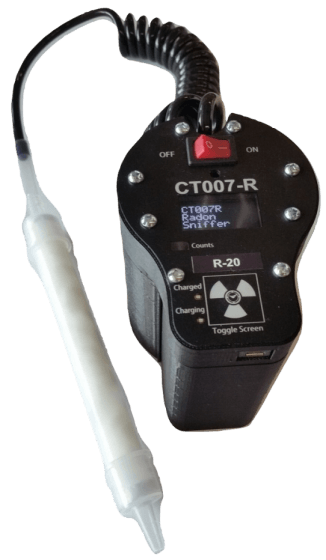
\includegraphics[scale=0.4]{images/CT007R.png}
\end{columns}


\end{frame}
\subsection{Problem Statement}
\begin{frame}{Problem Statement}
    Find a sampling schedule and algorithm to determine the concentrations of Rn-222 and Rn-220 that minimizes the variance in the estimated values of their concentrations.
\end{frame}
\section{Modelling}
\subsection{Linear Regression}
\begin{frame}{Linear Regression}
    Using the expected number of decays and the observed counts, we use a linear regression model to estimate the initial amount of each isotope. Thus we can fit the model:
    \begin{align*}
        y_i &= N_{222} {x_1}_i + N_{220} {x_2}_i + {\epsilon}_i
    \end{align*}
This allows us to estimate $N_{222}$ and $N_{220}$ when given a sample vector $y$ and inputs $X$ where $X=[{x}_1, {x}_2]$ as
\begin{align*}
    \begin{bmatrix}
    \hat{N}_{222}\\
    \hat{N}_{220}
    \end{bmatrix} = (X^TX)^{-1}X^T y
\end{align*}
\end{frame}
\begin{frame}{Decay Chains}
We model the decay chain as an ordered sequence of nuclides. These nuclides decay either by emitting an alpha particle or a beta particle, with a half-life of $t_{1/2}$. \\

\begin{columns}

\column{0.5\textwidth}
\begin{center}
\scalebox{0.4}{
\begin{tikzpicture}
    \node (Rn222) [rn] at (0,0) { $\underset{(3.825\,\mathrm{d}) }{ { }^{222}\mathrm{Rn} } $ };
    \node (Po218) [po] at (0,-3) { $\underset{(3.05\,\mathrm{min}) }{ { }^{218}\mathrm{Po} } $ };
    \node (Pb214) [pb] at (0,-6) { $\underset{(26.8\,\mathrm{min}) }{ { }^{214}\mathrm{Pb} } $ };
    \node (Bi214) [bi] at (3,-4.5) { $\underset{(19.7\,\mathrm{min}) }{ { }^{214}\mathrm{Bi} } $ };
    \node (Po214) [po] at (6,-3) { $\underset{(150\,\mu\mathrm{s}) }{ { }^{214}\mathrm{Po} } $ };
    \node (Pb210) [pb] at (6,-6) { $\underset{(22\,\mathrm{y}) }{ { }^{210}\mathrm{Pb} } $ };
    \node (At218) [at_ig] at (3,-1.5) { $\underset{(1.3\,\mathrm{s}) }{ { }^{218}\mathrm{At} } $ };
    \node (Tl210) [tl_ig] at (3,-7.5) { $\underset{(1.32\,\mathrm{min}) }{ { }^{210}\mathrm{Tl} } $ };
    \draw[very thick, ->] (Rn222) -- node[anchor=west] {$\alpha$} (Po218);
    \draw[very thick,->] (Po218) -- node[anchor=west] {$\alpha$} (Pb214);
    \draw[very thick,->] (Pb214) -- node[anchor=north west] {$\beta$} (Bi214);
    \draw[very thick,->] (Bi214) -- node[anchor=north west] {$\beta$} (Po214);
    \draw[very thick,->] (Po214) -- node[anchor=west] {$\alpha$} (Pb210);
    \draw[black!40,->] (Po218) -- node[anchor=north west] {$\underset{0.03\%}{\beta} $} (At218);
    \draw[black!40,->] (At218) -- node[anchor=west] {$\alpha$} (Bi214);
    \draw[black!40,->] (Bi214) -- node[anchor=west] {$\underset{0.04\%}{\alpha} $} (Tl210);
    \draw[black!40,->] (Tl210) -- node[anchor=north west] {$\beta $} (Pb210);
\end{tikzpicture}
}
\end{center}
\column{0.5\textwidth}
\begin{center}
\scalebox{0.4}{
\begin{tikzpicture}
    \node (Rn220) [rn] at (0,0) { $\underset{(54.5\,\mathrm{s})}{ { }^{220}\mathrm{Rn} } $ };
    \node (Po216) [po] at (0,-3) { $\underset{(0.158\,\mathrm{s})}{ { }^{216}\mathrm{Po} } $ };
    \node (Pb212) [pb] at (0,-6) { $\underset{(10.6\,\mathrm{h})}{ { }^{212}\mathrm{Pb} } $ };
    \node (Bi212) [bi] at (3,-4.5) { $\underset{(60.5\,\mathrm{min})}{ { }^{212}\mathrm{Bi} } $ };
    \node (Po212) [po_ig] at (6,-3) { $\underset{(0.3\,\mu\mathrm{s})}{ { }^{212}\mathrm{Po} } $ };
    \node (Tl208) [tl_ig] at (3,-7.5) { $\underset{(3.1\,\mathrm{m})}{ { }^{208}\mathrm{Tl} } $ };
    \node (Pb208) [pb] at (6,-6) { $\underset{(\mathrm{stable})}{ { }^{208}\mathrm{Pb} } $ };
    \node (At216) [at_ig] at (3,-1.5) { $\underset{(300\,\mu\mathrm{s}) }{ { }^{216}\mathrm{At} } $ };
    \draw[very thick,->] (Rn220) -- node[anchor=west] {$\alpha$} (Po216);
    \draw[very thick,->] (Po216) -- node[anchor=west] {$\alpha$} (Pb212);
    \draw[very thick,->] (Pb212) -- node[anchor=north west] {$\beta$} (Bi212);
    \draw[black!40,->] (At216) -- node[anchor=west] {$\alpha$} (Bi212);
    \draw[black!40,->] (Po216) -- node[anchor=north west] {$\underset{0.013\%}{\beta}$} (At216);
    \draw[black!40,->] (Bi212) -- node[anchor=north west] {$\underset{66.3\%}{\beta}$} (Po212);
    \draw[black!40,->] (Bi212) -- node[anchor=west] {$\alpha$} (Tl208);
    \draw[black!40,->] (Po212) -- node[anchor=west] {$\alpha$} (Pb208);
    \draw[black!40,->] (Tl208) -- node[anchor=north west] {$\underset{33.7\%}{\beta}$} (Pb208);
    \draw[very thick,->] (Bi212) -- node[anchor=north east] {$\approx \alpha $} (Pb208);
\end{tikzpicture}
}
\end{center}
\end{columns}
% Radon 222:
% \footnotesize{
% \[
%      {}^{222}\mathrm{Rn} \xrightarrow{\alpha,\; 3.825 d} {}^{218}\mathrm{Po} \xrightarrow{\alpha,\; 3.05 m} {}^{214}\mathrm{Pb} \xrightarrow{\beta, \; 26.8 m} {}^{214}\mathrm{Bi} \xrightarrow{\beta, \; 19.7 m} {}^{214}\mathrm{Po} \xrightarrow{\alpha, \; 150 \mu s} {}^{210}\mathrm{Pb}
% \]

% }
% \normalsize
% Thoron (Radon 220):

% \footnotesize{
% \[
% {}^{220}\mathrm{Rn} \xrightarrow{\alpha,\: 54.5 s} { }^{216}\mathrm{Po} \xrightarrow{\alpha, \; 0.158 s} {}^{212}\mathrm{Pb} \xrightarrow{\beta, \; 10.6 h} { }^{212}\mathrm{Bi} \xrightarrow{\approx \alpha, \; \approx 60.5 m} { }^{208}\mathrm{Pb}
% \]

% }
\end{frame}

\subsection{Bateman Equation}

\begin{frame}{Decay Rate}
    For a collection of $N(0)$ unstable atoms, all of a single nuclide,
    the number $N(t)$ of atoms \textit{expected} to be remaining at time $t$ is given by
    \[ N(t)=N(0)e^{-\lambda t} \]
    for a value $\lambda>0$ called the \textit{decay constant} for that nuclide.\\
    \vspace{0.2cm}
    The expected rate of decay at time $t$ is given by
    \[ -\frac{dN}{dt}=\lambda N(t). \]
\end{frame}

\begin{frame}{System of ODEs}
%The formula for the *expected* number $N(t)$ of atoms remaining undecayed at time $t$ is
%$$
%    N(t): = N_0e^{-\lambda t}.
%$$
%Because of this, the expected decay rate of atoms at time $t$ is
%$$
%    \frac{dN}{dt}(t) = -\lambda N(t).
%$$
  Let $N_0(t),N_1(t),\ldots,N_\ell(t)$ denote the expected number of atoms of each type in a given decay chain remaining at time $t$.
  Let $\lambda_j$ denote the decay constant of the $j$-th member of the chain.
%When $0<j<\ell$, the number $N_j(t)$ can change over time either by the decay of an atom of time $X_j$ into one of type $X_{j+1}$ (decreasing $N_j(t)$ in the process) or by an atom of $X_{j-1}$ decaying into an atom of $X_j$ (therby increasing $N_j(t)$.
%This gives rise to the differential equation
%By the rates of creation to those of decay for a given nuclide in the chain,
%one finds that t
The evolution of the system is described by the following ODEs:
$$
    \frac{dN_0}{dt}=-\lambda_0 N_0, \quad \frac{dN_j}{dt} = -\lambda_j N_j + \lambda_{j-1}N_{j-1} \quad (0<j \leq \ell)
$$
\end{frame}
\begin{frame}{Bateman Equation}
    Note that our detector does not measure $N_j(t)$ but instead a sum of expressions of the form 
    $$
    \int_{s_1}^{s_2}\lambda_j N_j(s)ds,
    $$
where $(s_1,s_2]$ is an interval of time during which the detector is counting.
Nevertheless, it will be in our interest to solve for $N_j$ first.\\
\vspace{0.2cm}
The solutions of the system are provided by the \textit{Bateman Equation} when $N_1(0)=\cdots=N_\ell(0)=0$:
$$
    N_j(t) = \frac{N_0(0)}{\lambda_j}\sum_{r=0}^j\left(\prod_{q=0,q\neq r}^j \frac{\lambda_q}{\lambda_q-\lambda_r}\right)\lambda_r e^{-\lambda_r t}.
$$
\end{frame}

\begin{frame}{Bateman Equation}
    Thus the number of decays by atoms of the $j$-th type in the time interval $(s_1,s_2]$ is
$$
    \int_{s_1}^{s_2} \lambda_j N_j(s)ds = N_0(0)\sum_{r=0}^j\left(\prod_{q=0,q\neq r}^j \frac{\lambda_q}{\lambda_q-\lambda_r}\right)(e^{-\lambda_r s_1}-e^{-\lambda_r s_2})
$$  

Since our detector only detects alpha decays,
the number of counts we expect to see in the time interval $(s_1,s_2]$ is given by by
$$
    \sum_{j \: \alpha\text{-decays}}\int_{s_1}^{s_2}\lambda_j N_j(s)ds.
$$
\end{frame}
{\nologo
\begin{frame}{Normalized Count Rates}
Normalizing to the expected counts in the first sampling period, here equal to 1 second, we can see the difference in behaviour of different mixtures of radon and thoron.
    \begin{center}
        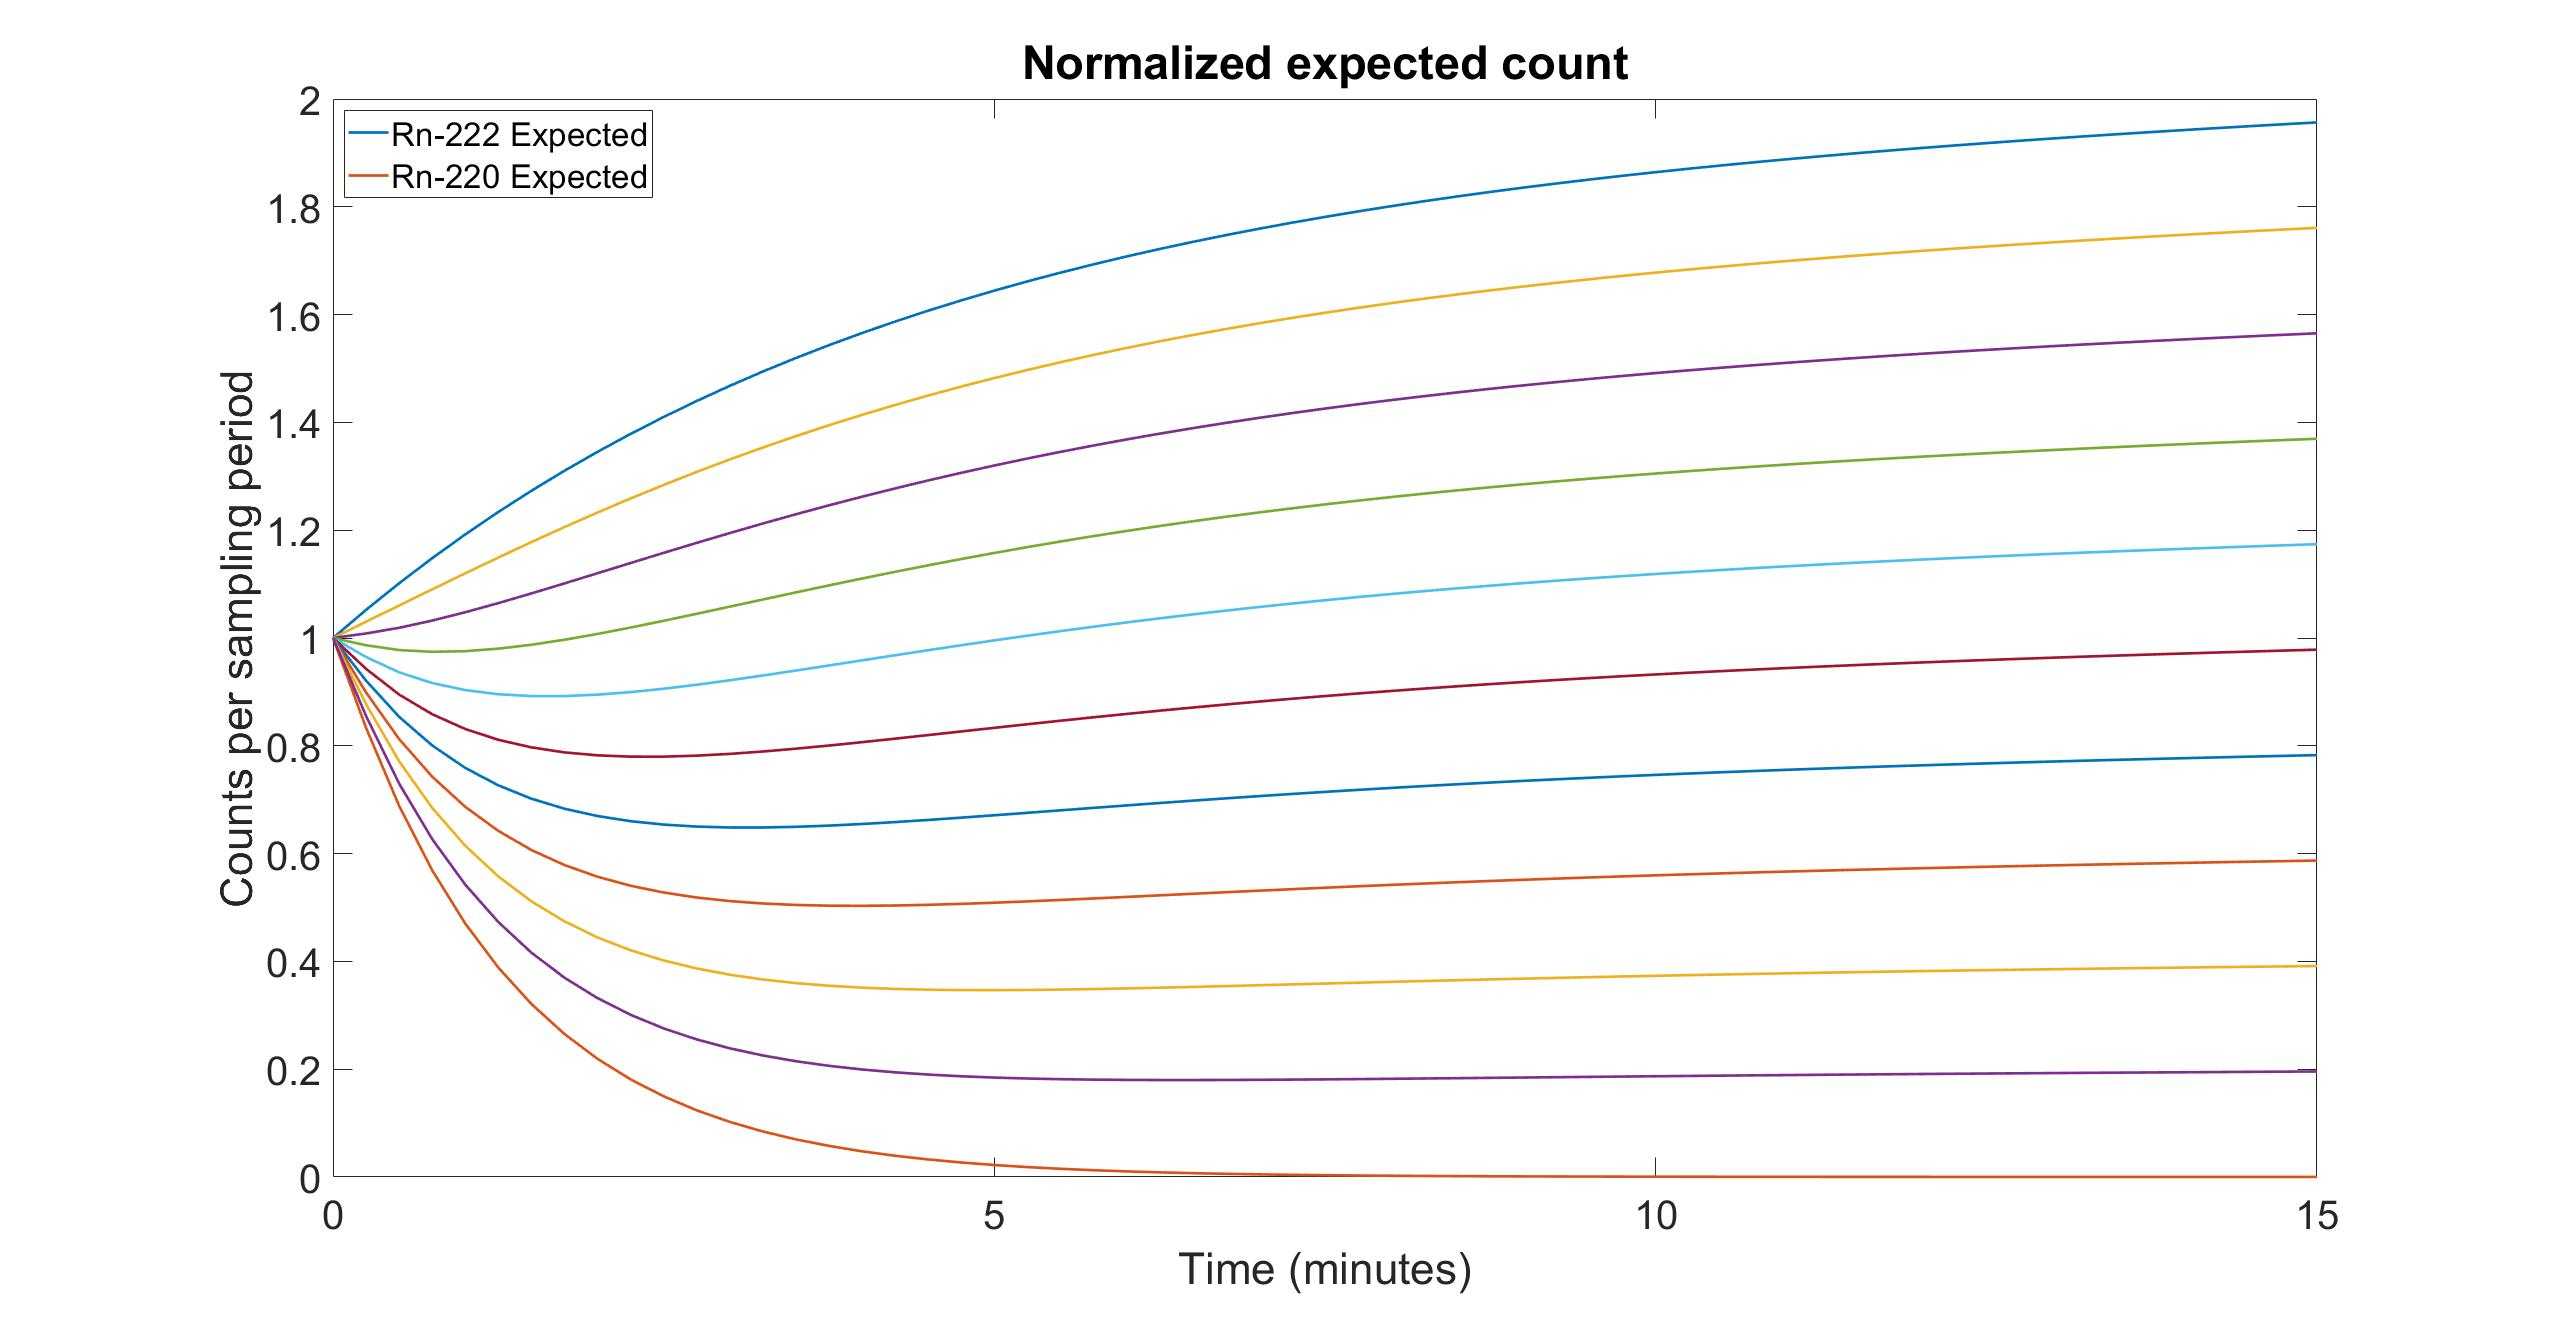
\includegraphics[width=\textwidth]{images/expected_counts.jpg}
        % \includegraphics[scale=0.45]{Normalized_Mixture_9.png}
    \end{center}
\end{frame}
}
\subsection{Generating Data}
\begin{frame}{Generating Data}
Since we are testing new sampling times and periods, and we have limited real world datasets to test our model with, we need to generate data that will simulate radon and thoron decay.\\
\vspace{0.2cm}
The decay times of an atom follow an exponential distribution with parameter $\lambda = \frac{\ln(2)}{t_{1/2}}$. From here we can follow the evolution of an atom along the decay chain.\\
\vspace{0.2cm}
%By sampling the decay time of the atoms of each nuclide from its distribution, and counting the total number of decays within a certain interval, we can generate simulated data. 
\begin{center}
    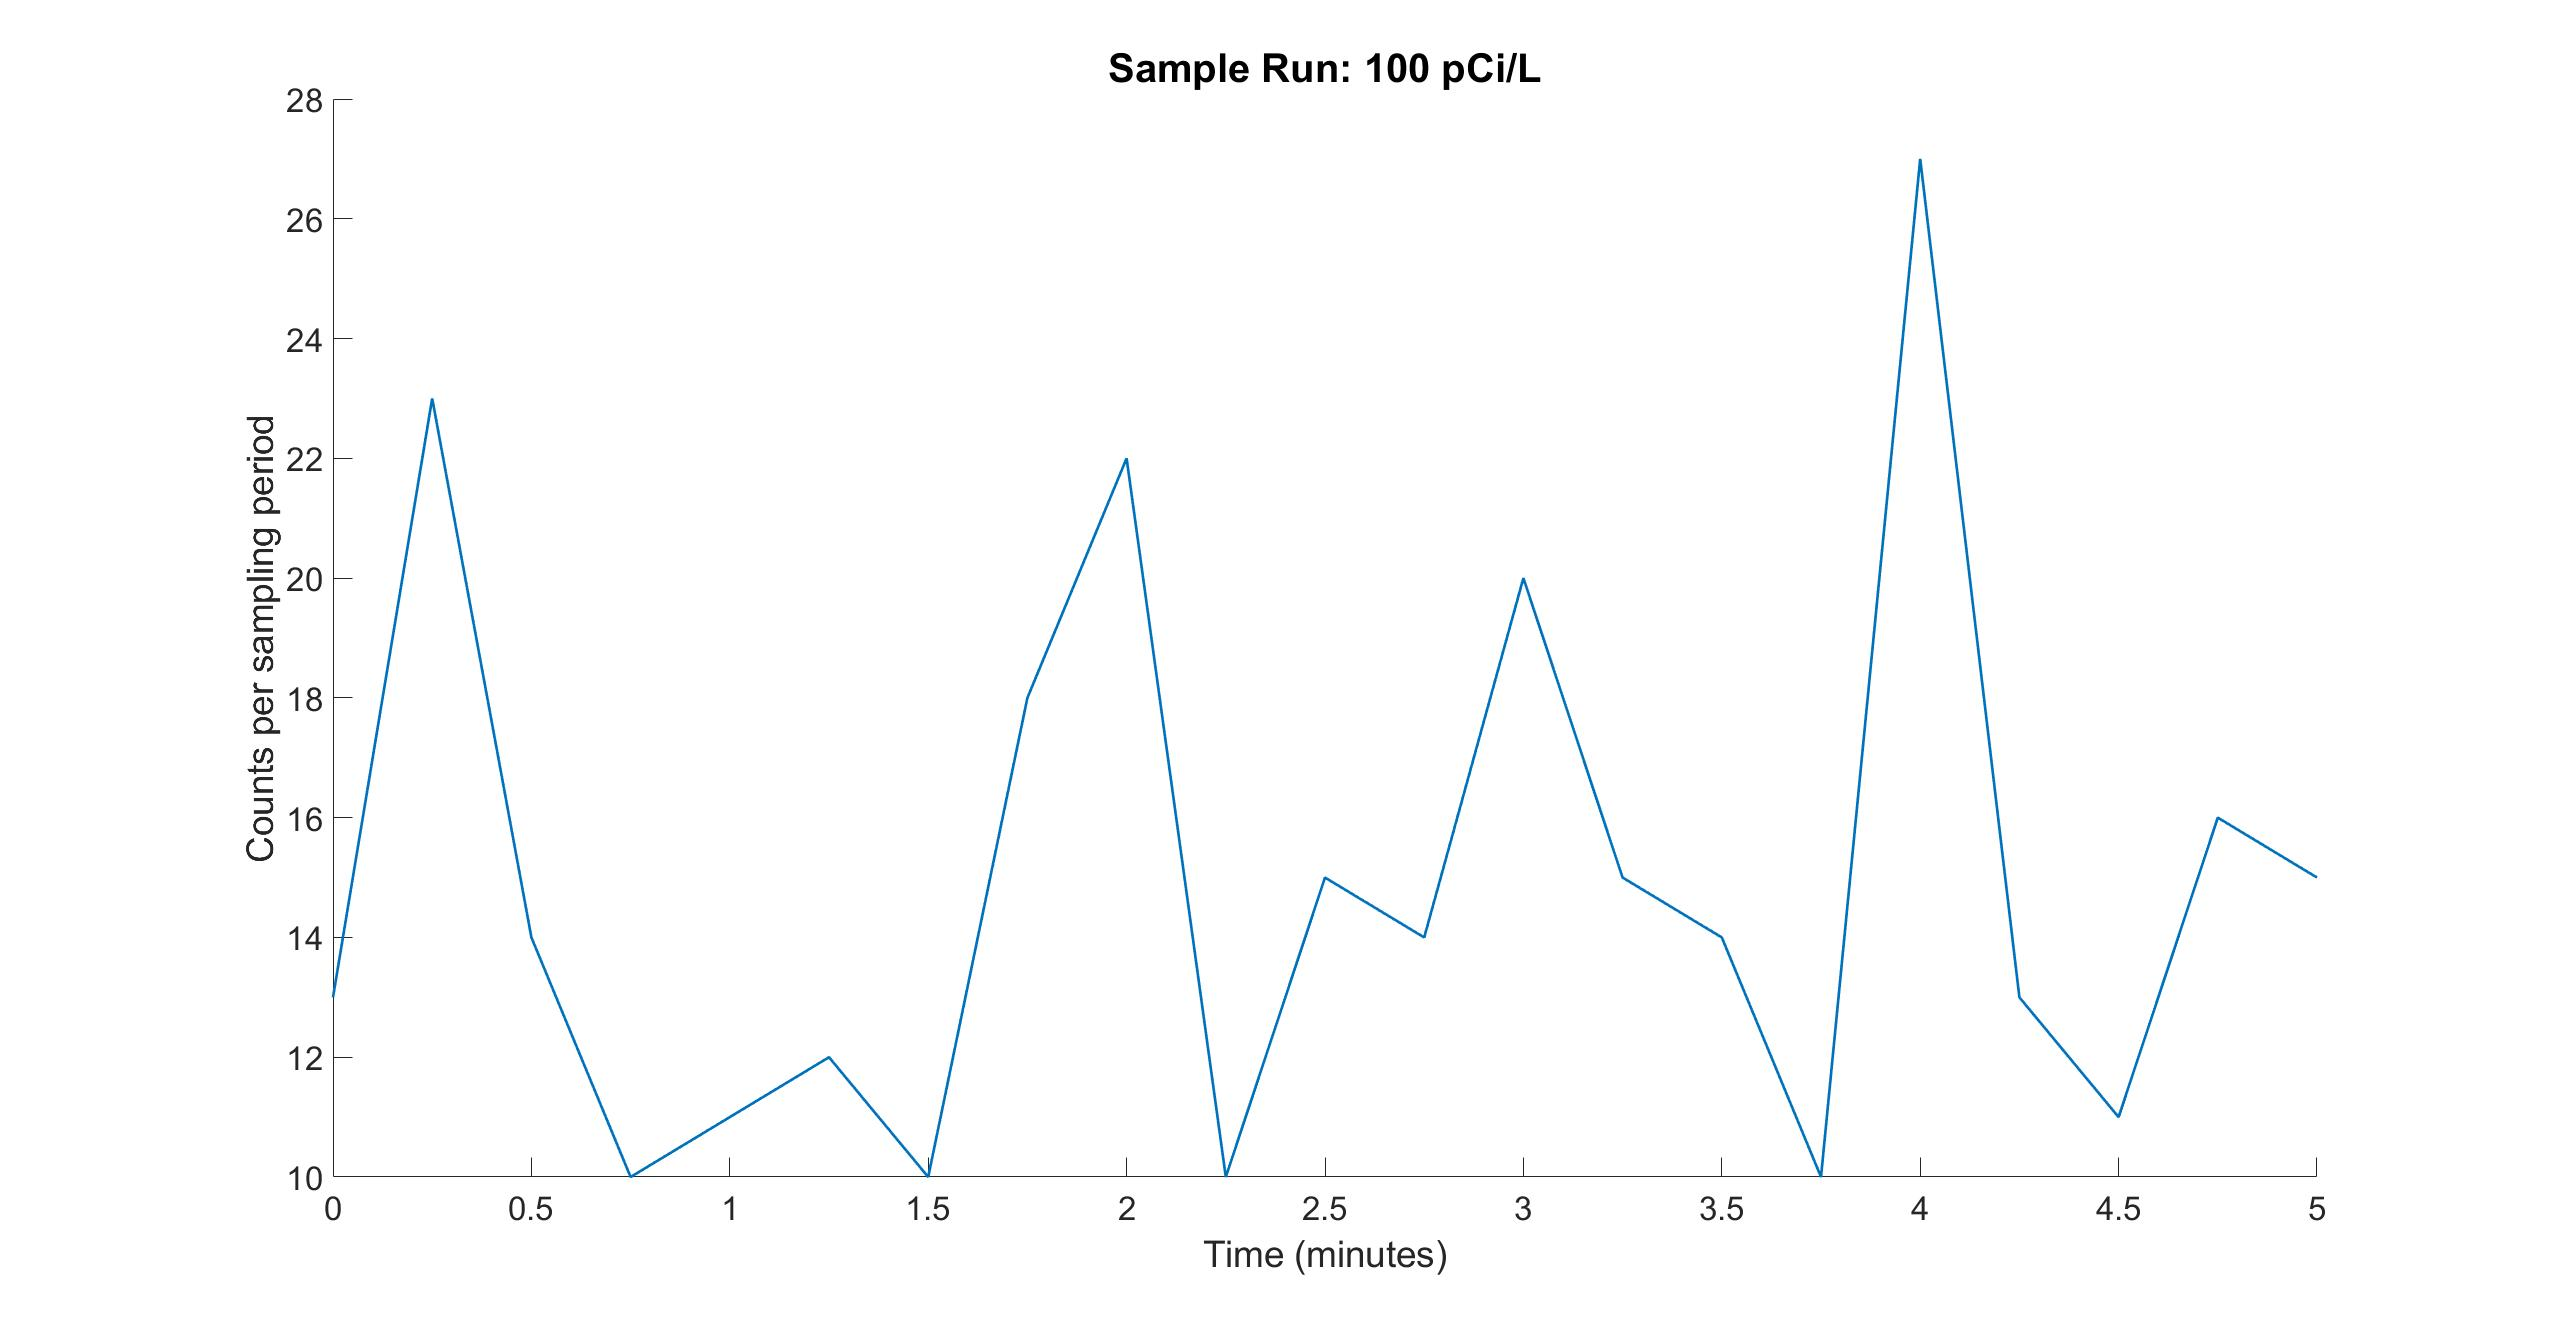
\includegraphics[scale=0.085]{images/samplerun.jpg}
\end{center}
\end{frame}
{\nologo
\begin{frame}{10 pCi/L}

    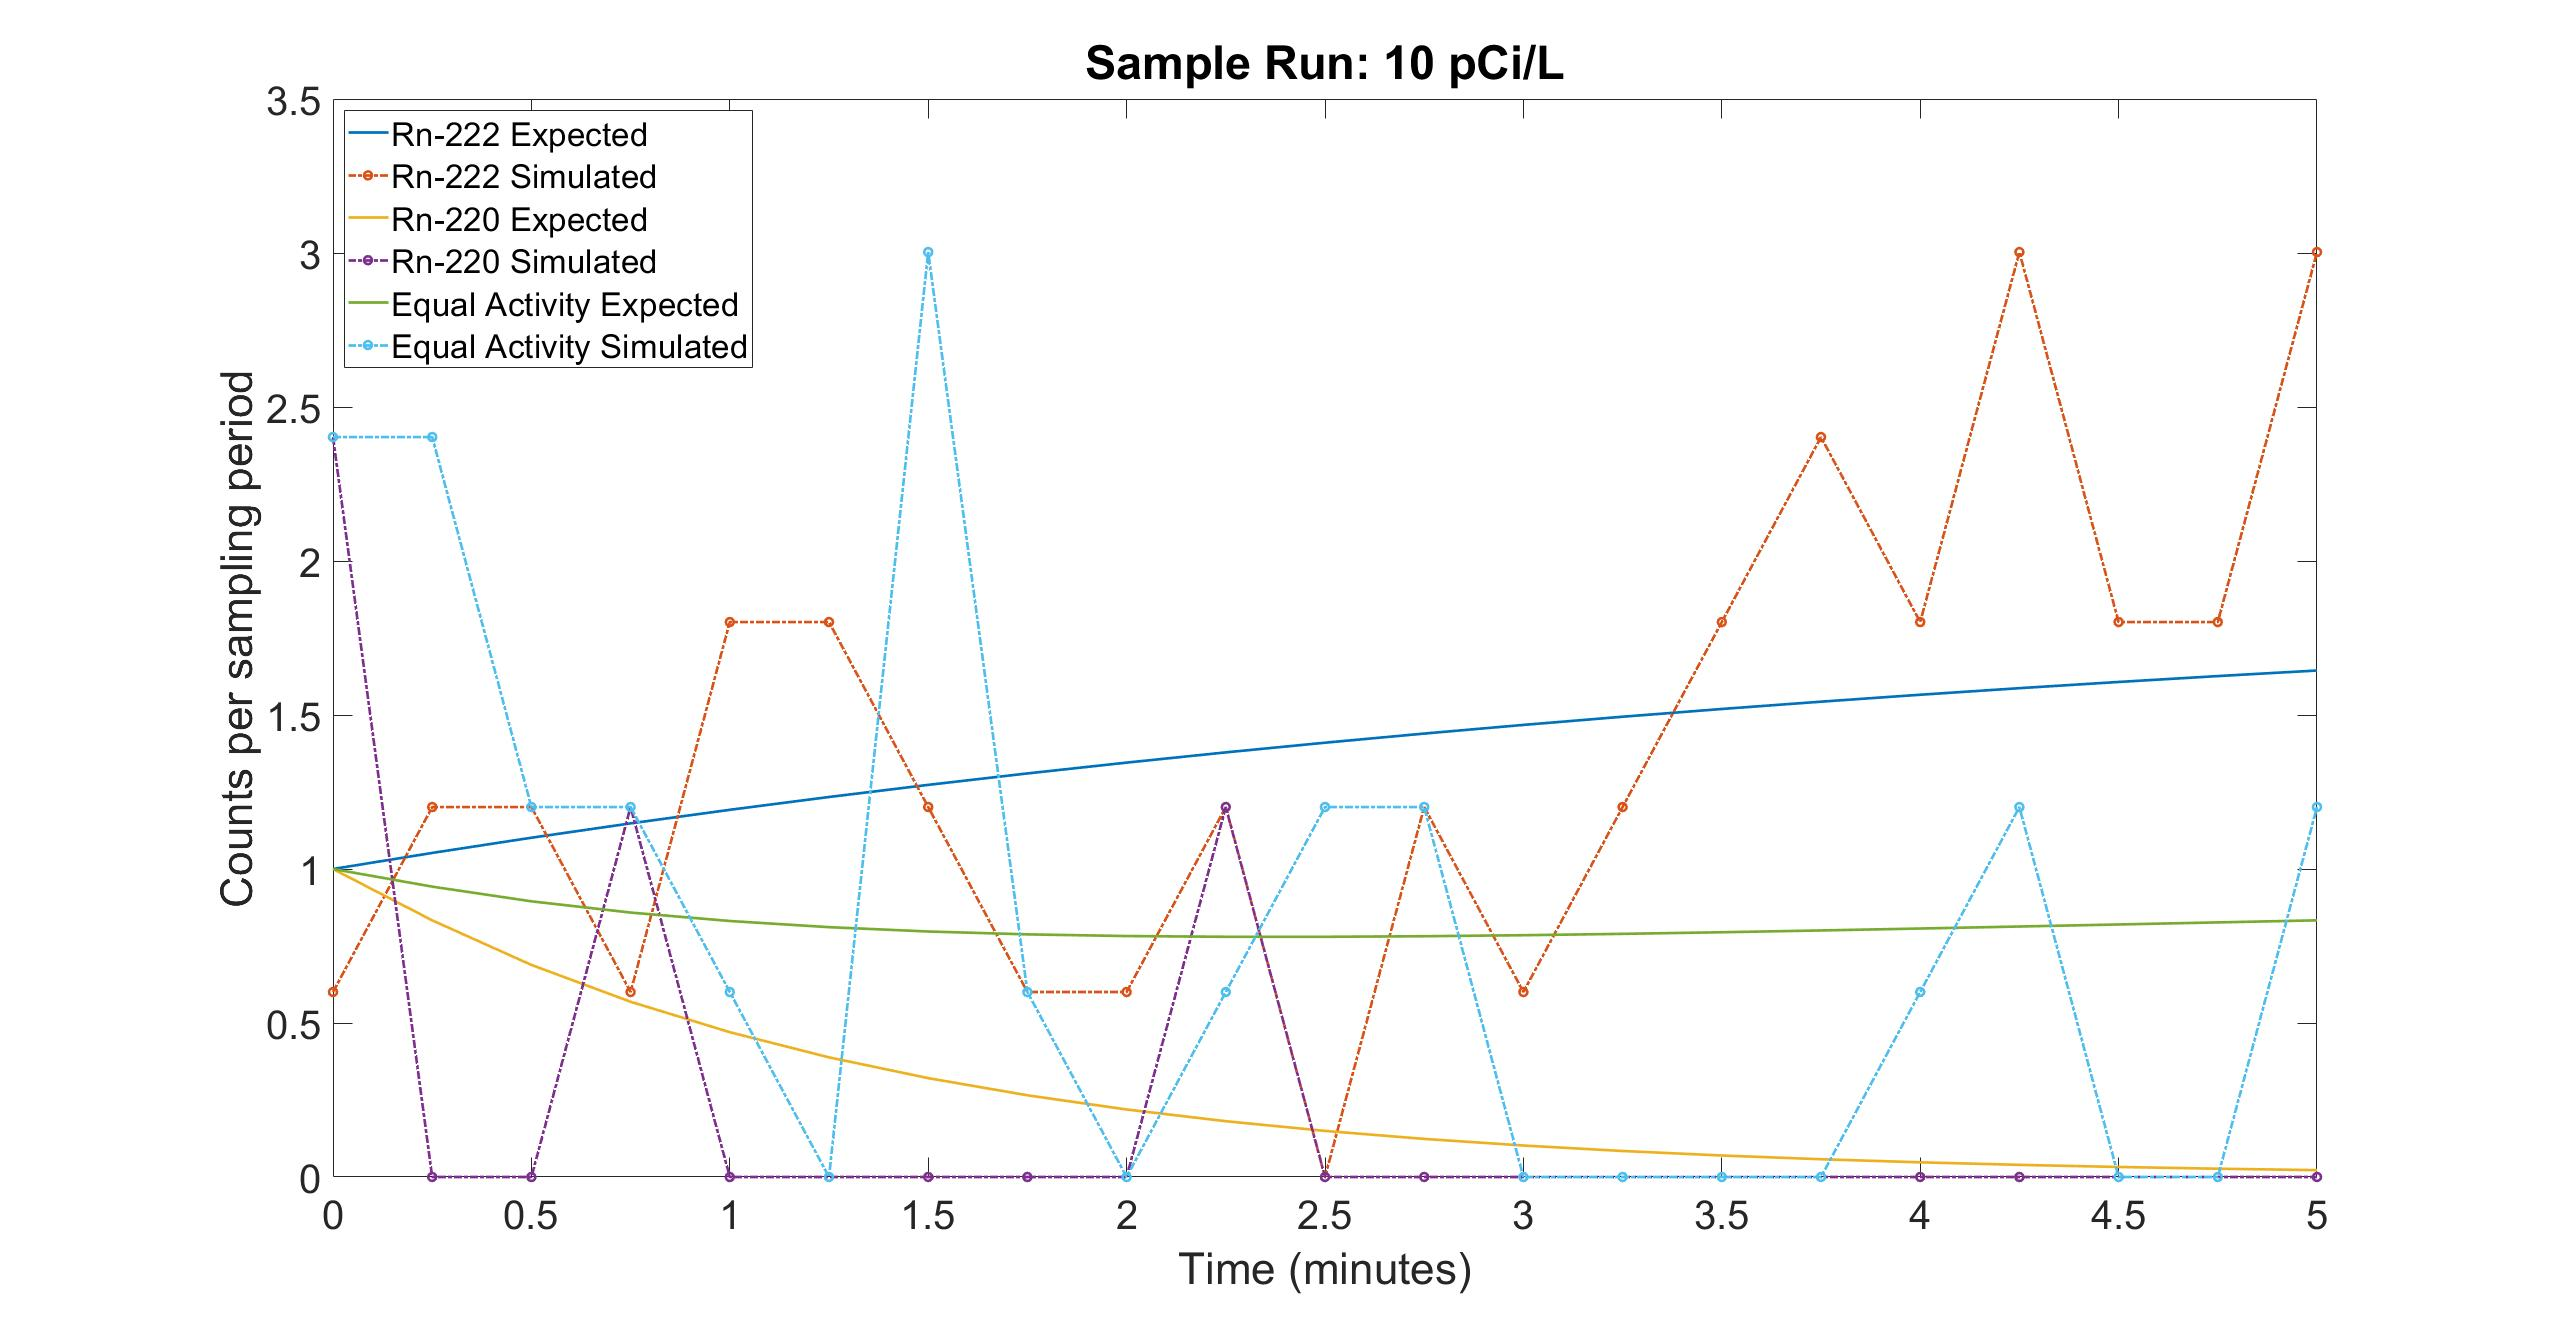
\includegraphics[width=\textwidth]{images/10pCipL.jpg}
    We can add a sample run of generated data onto the theoretical curves and compare the observed counts to the expected counts.
\end{frame}
\begin{frame}{100 pCi/L}
    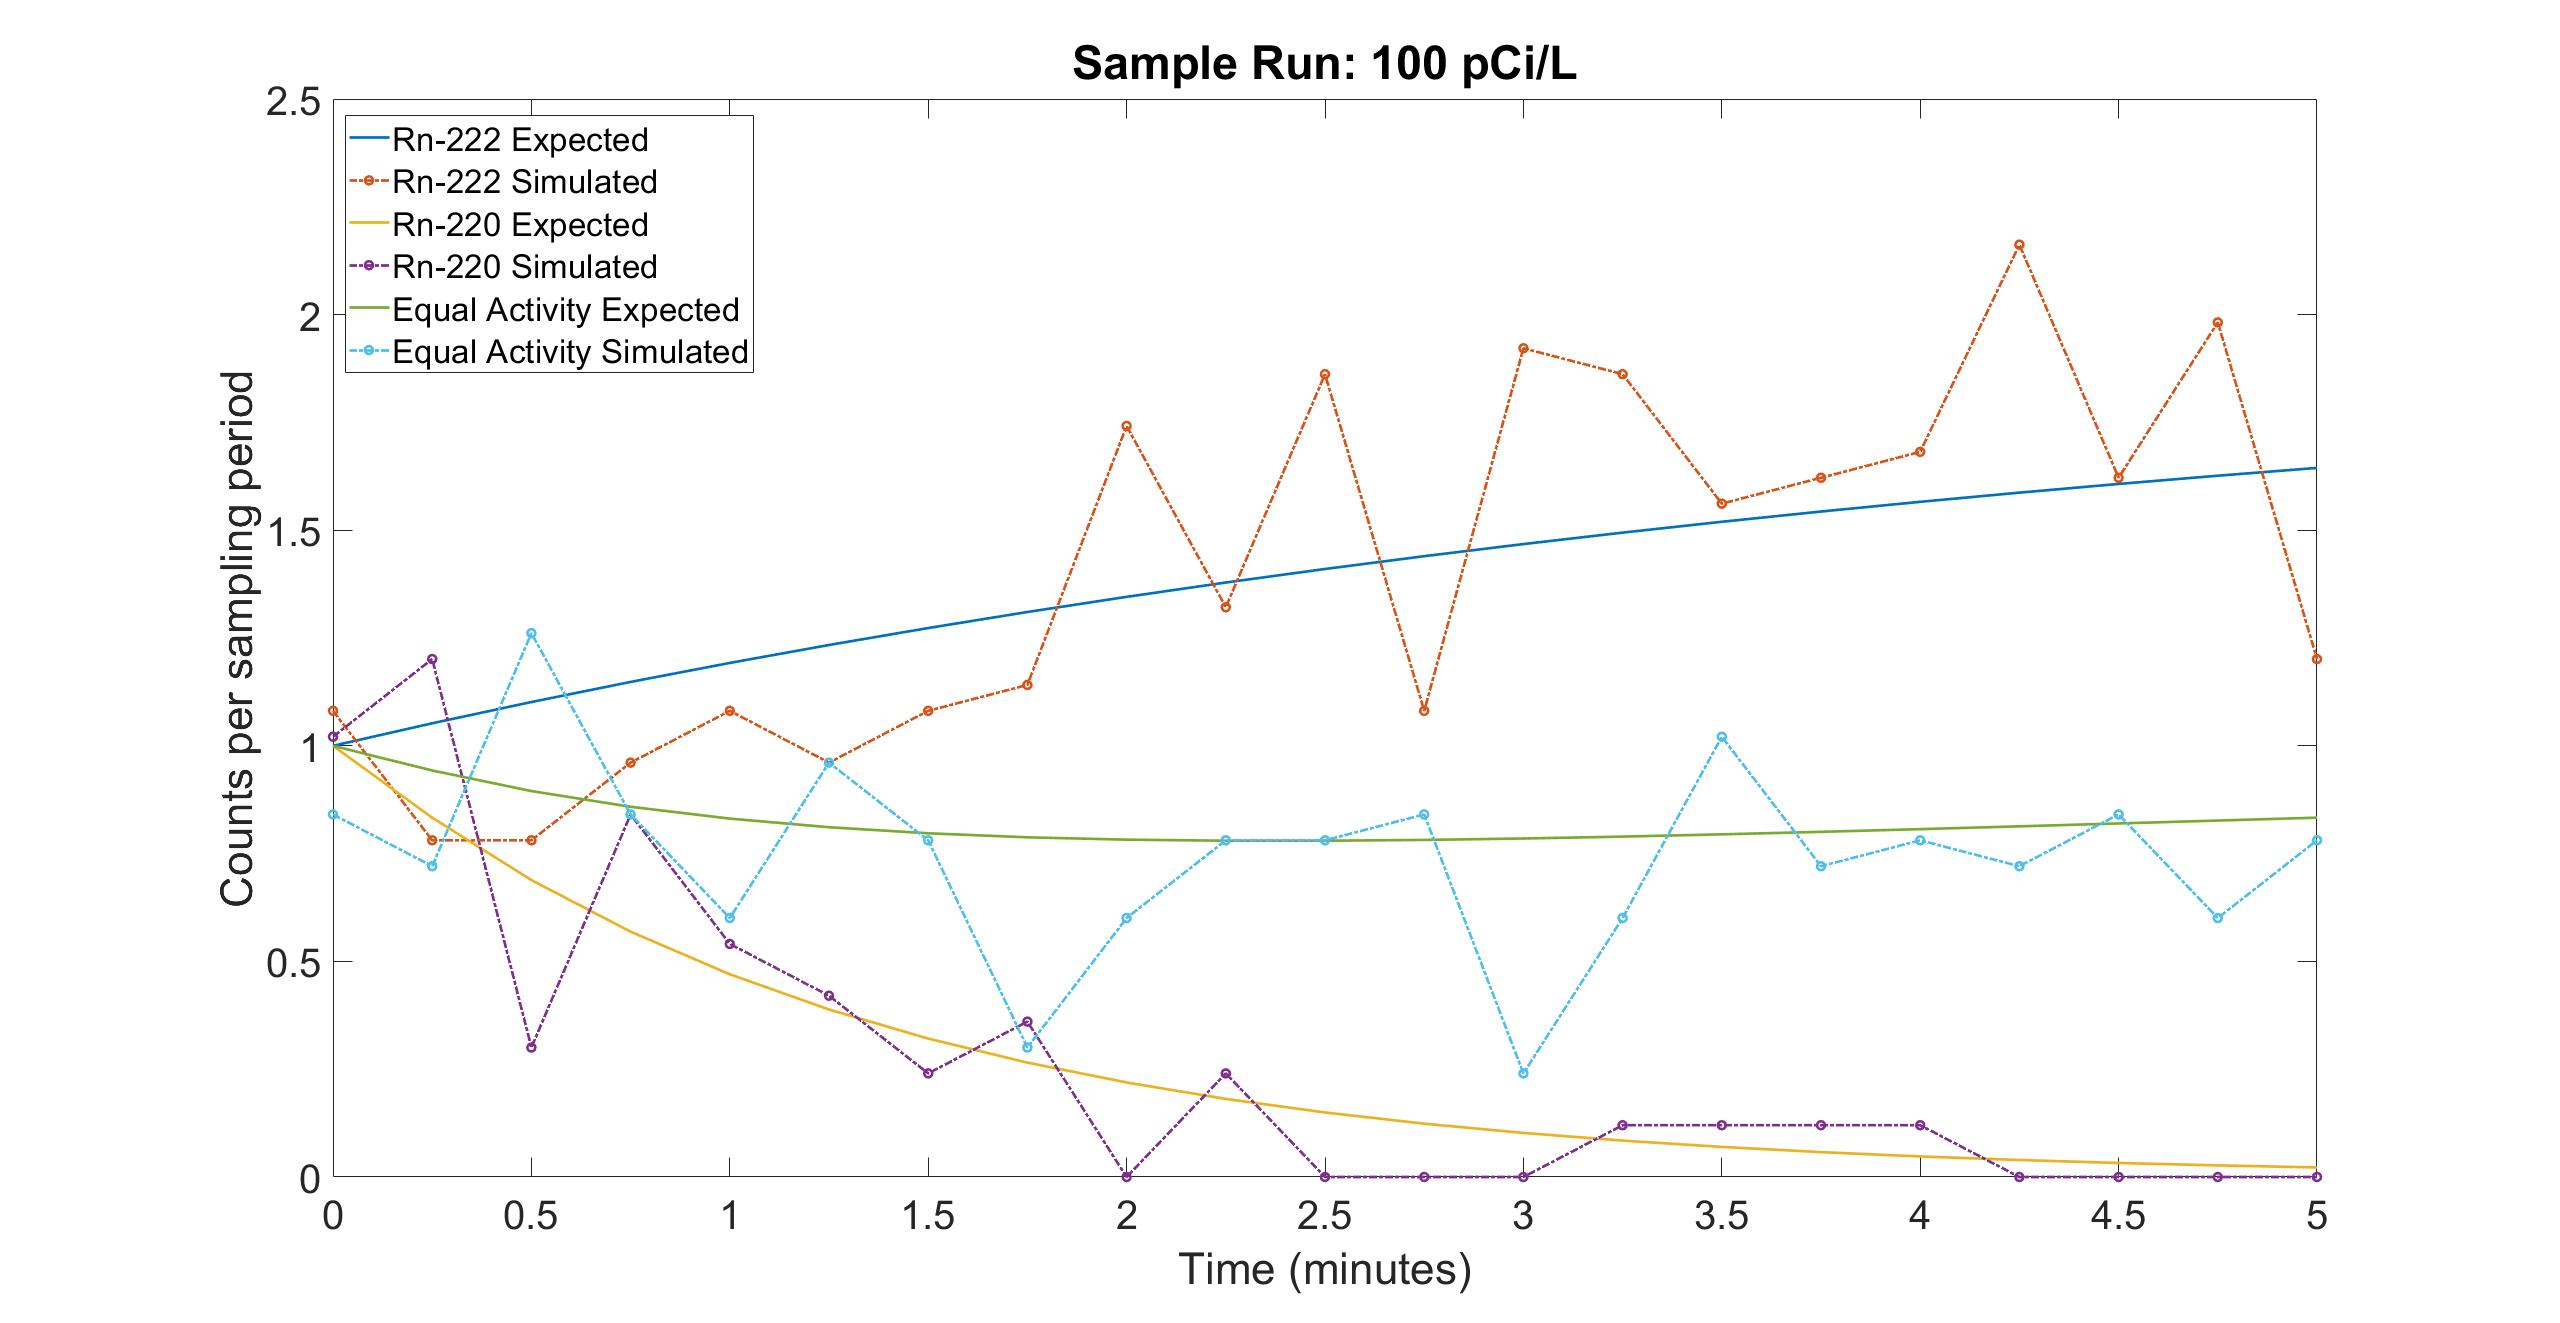
\includegraphics[width=\textwidth]{images/100pCipL.jpg}
\end{frame}
\begin{frame}{8000 pCi/L}
    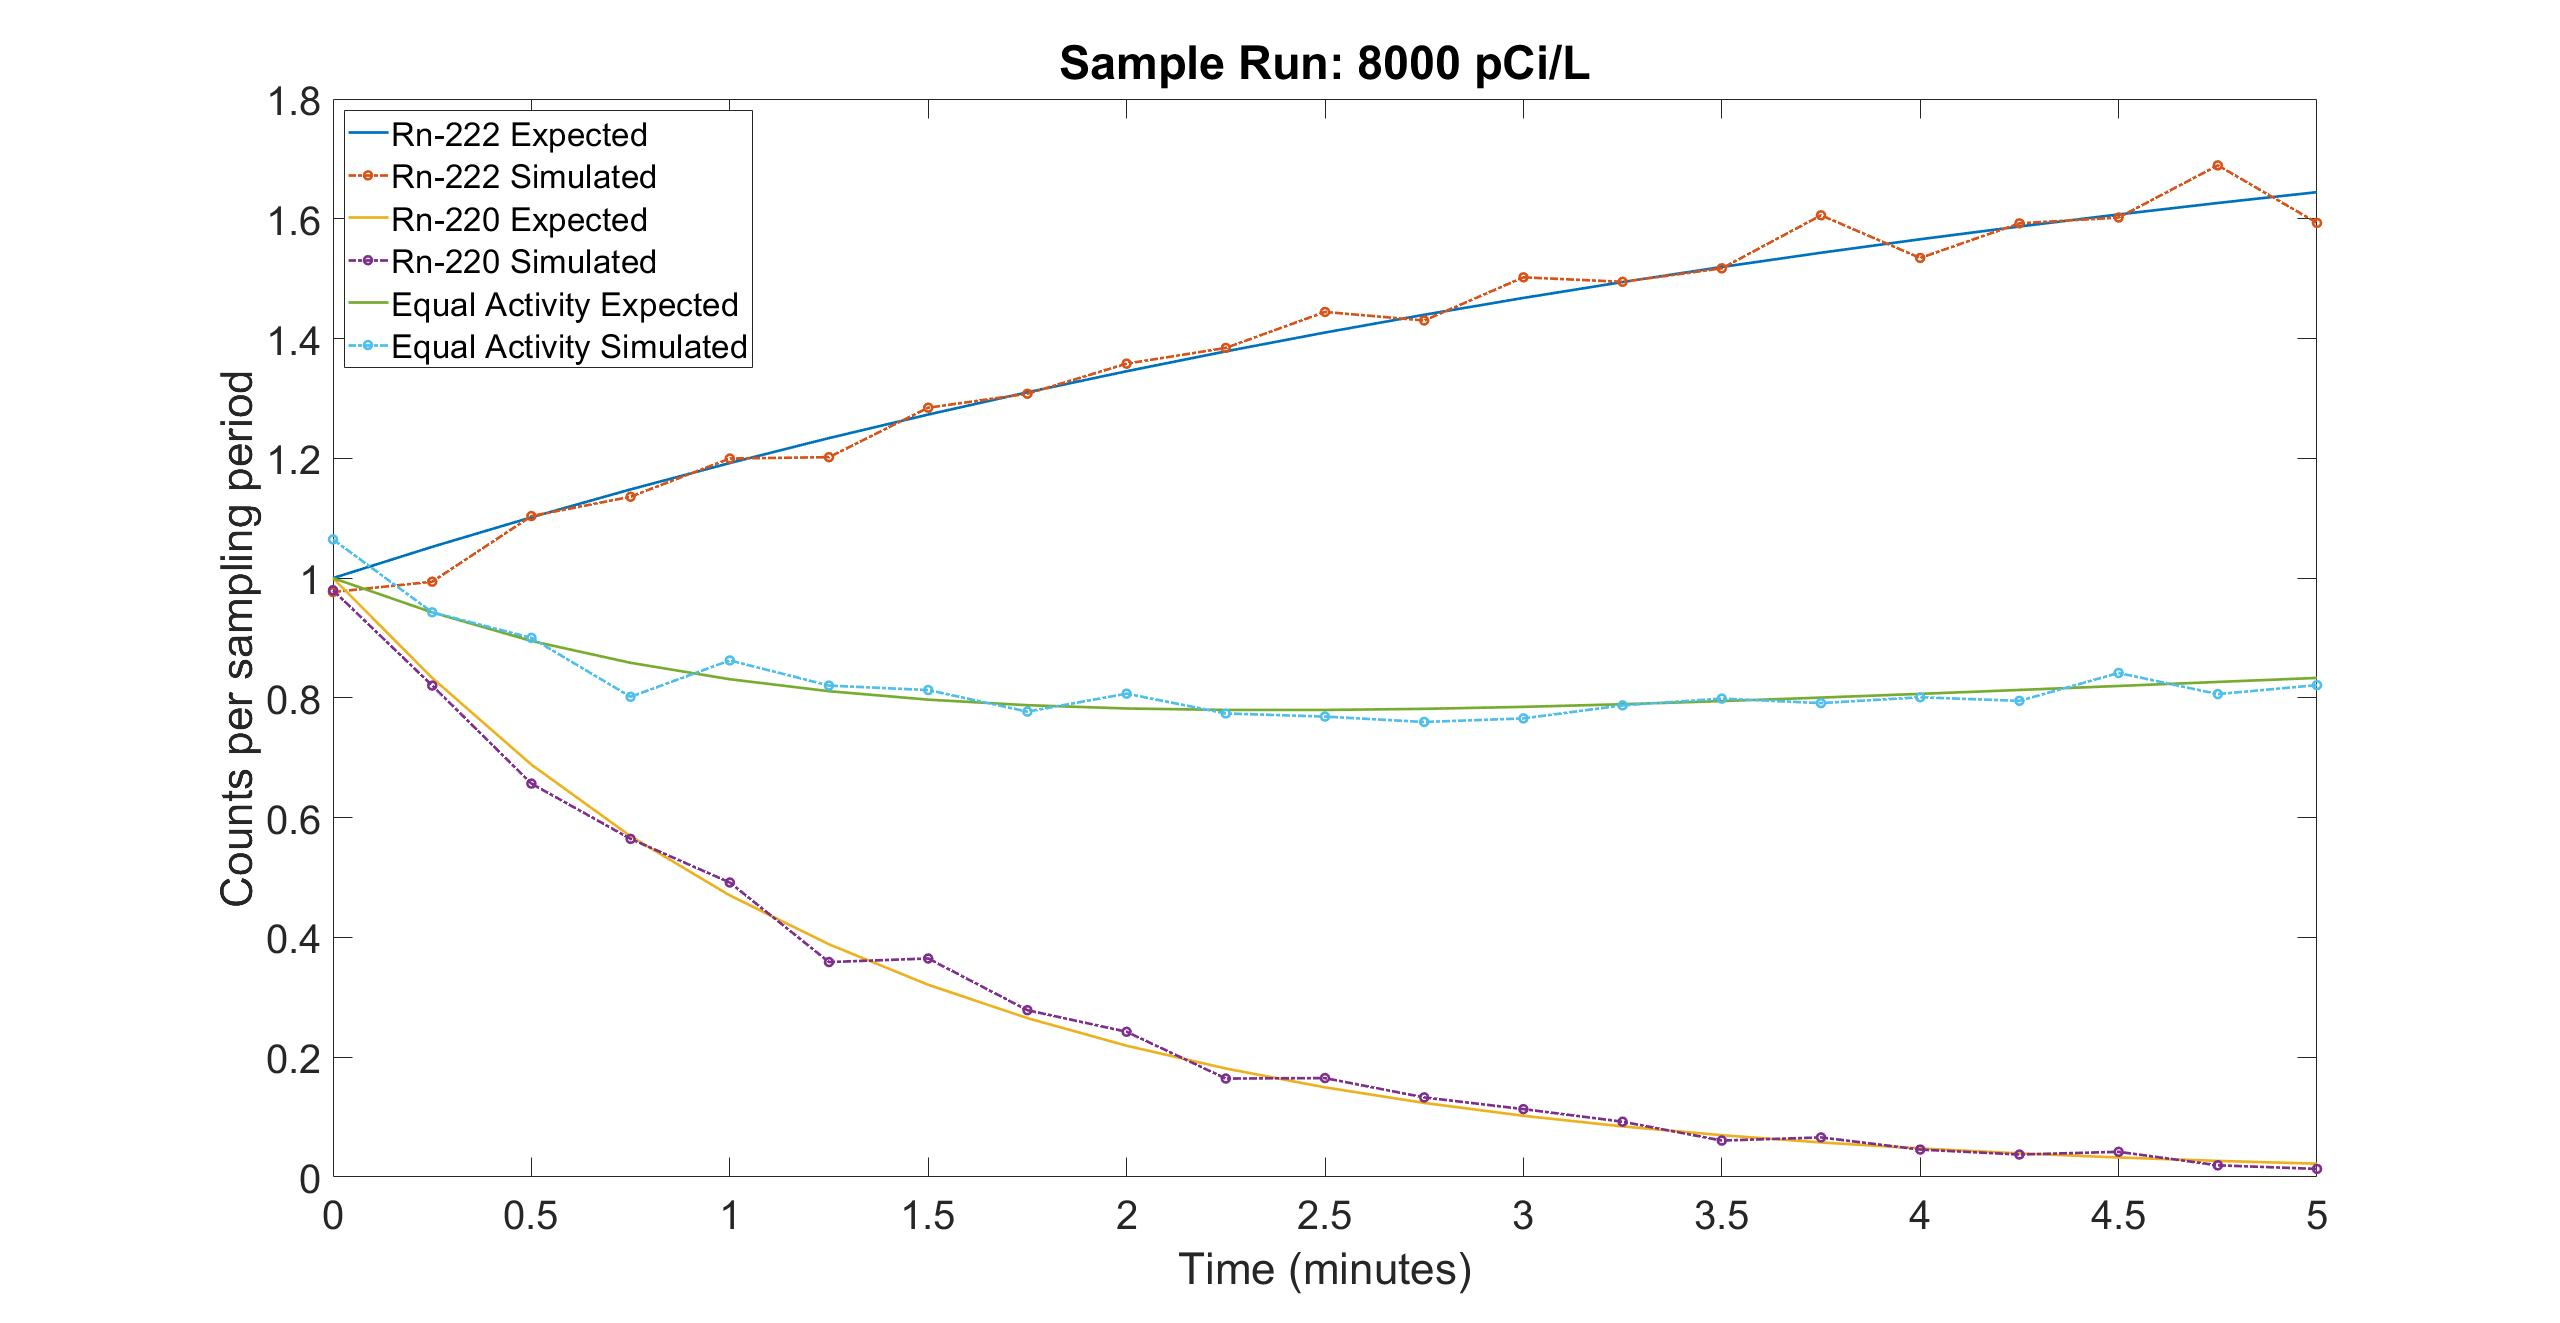
\includegraphics[width=\textwidth]{images/8000pCipL.jpg}
\end{frame}
}

\section{Results}
\subsection{Determined Coefficients}
\begin{frame}{Grid Search}
    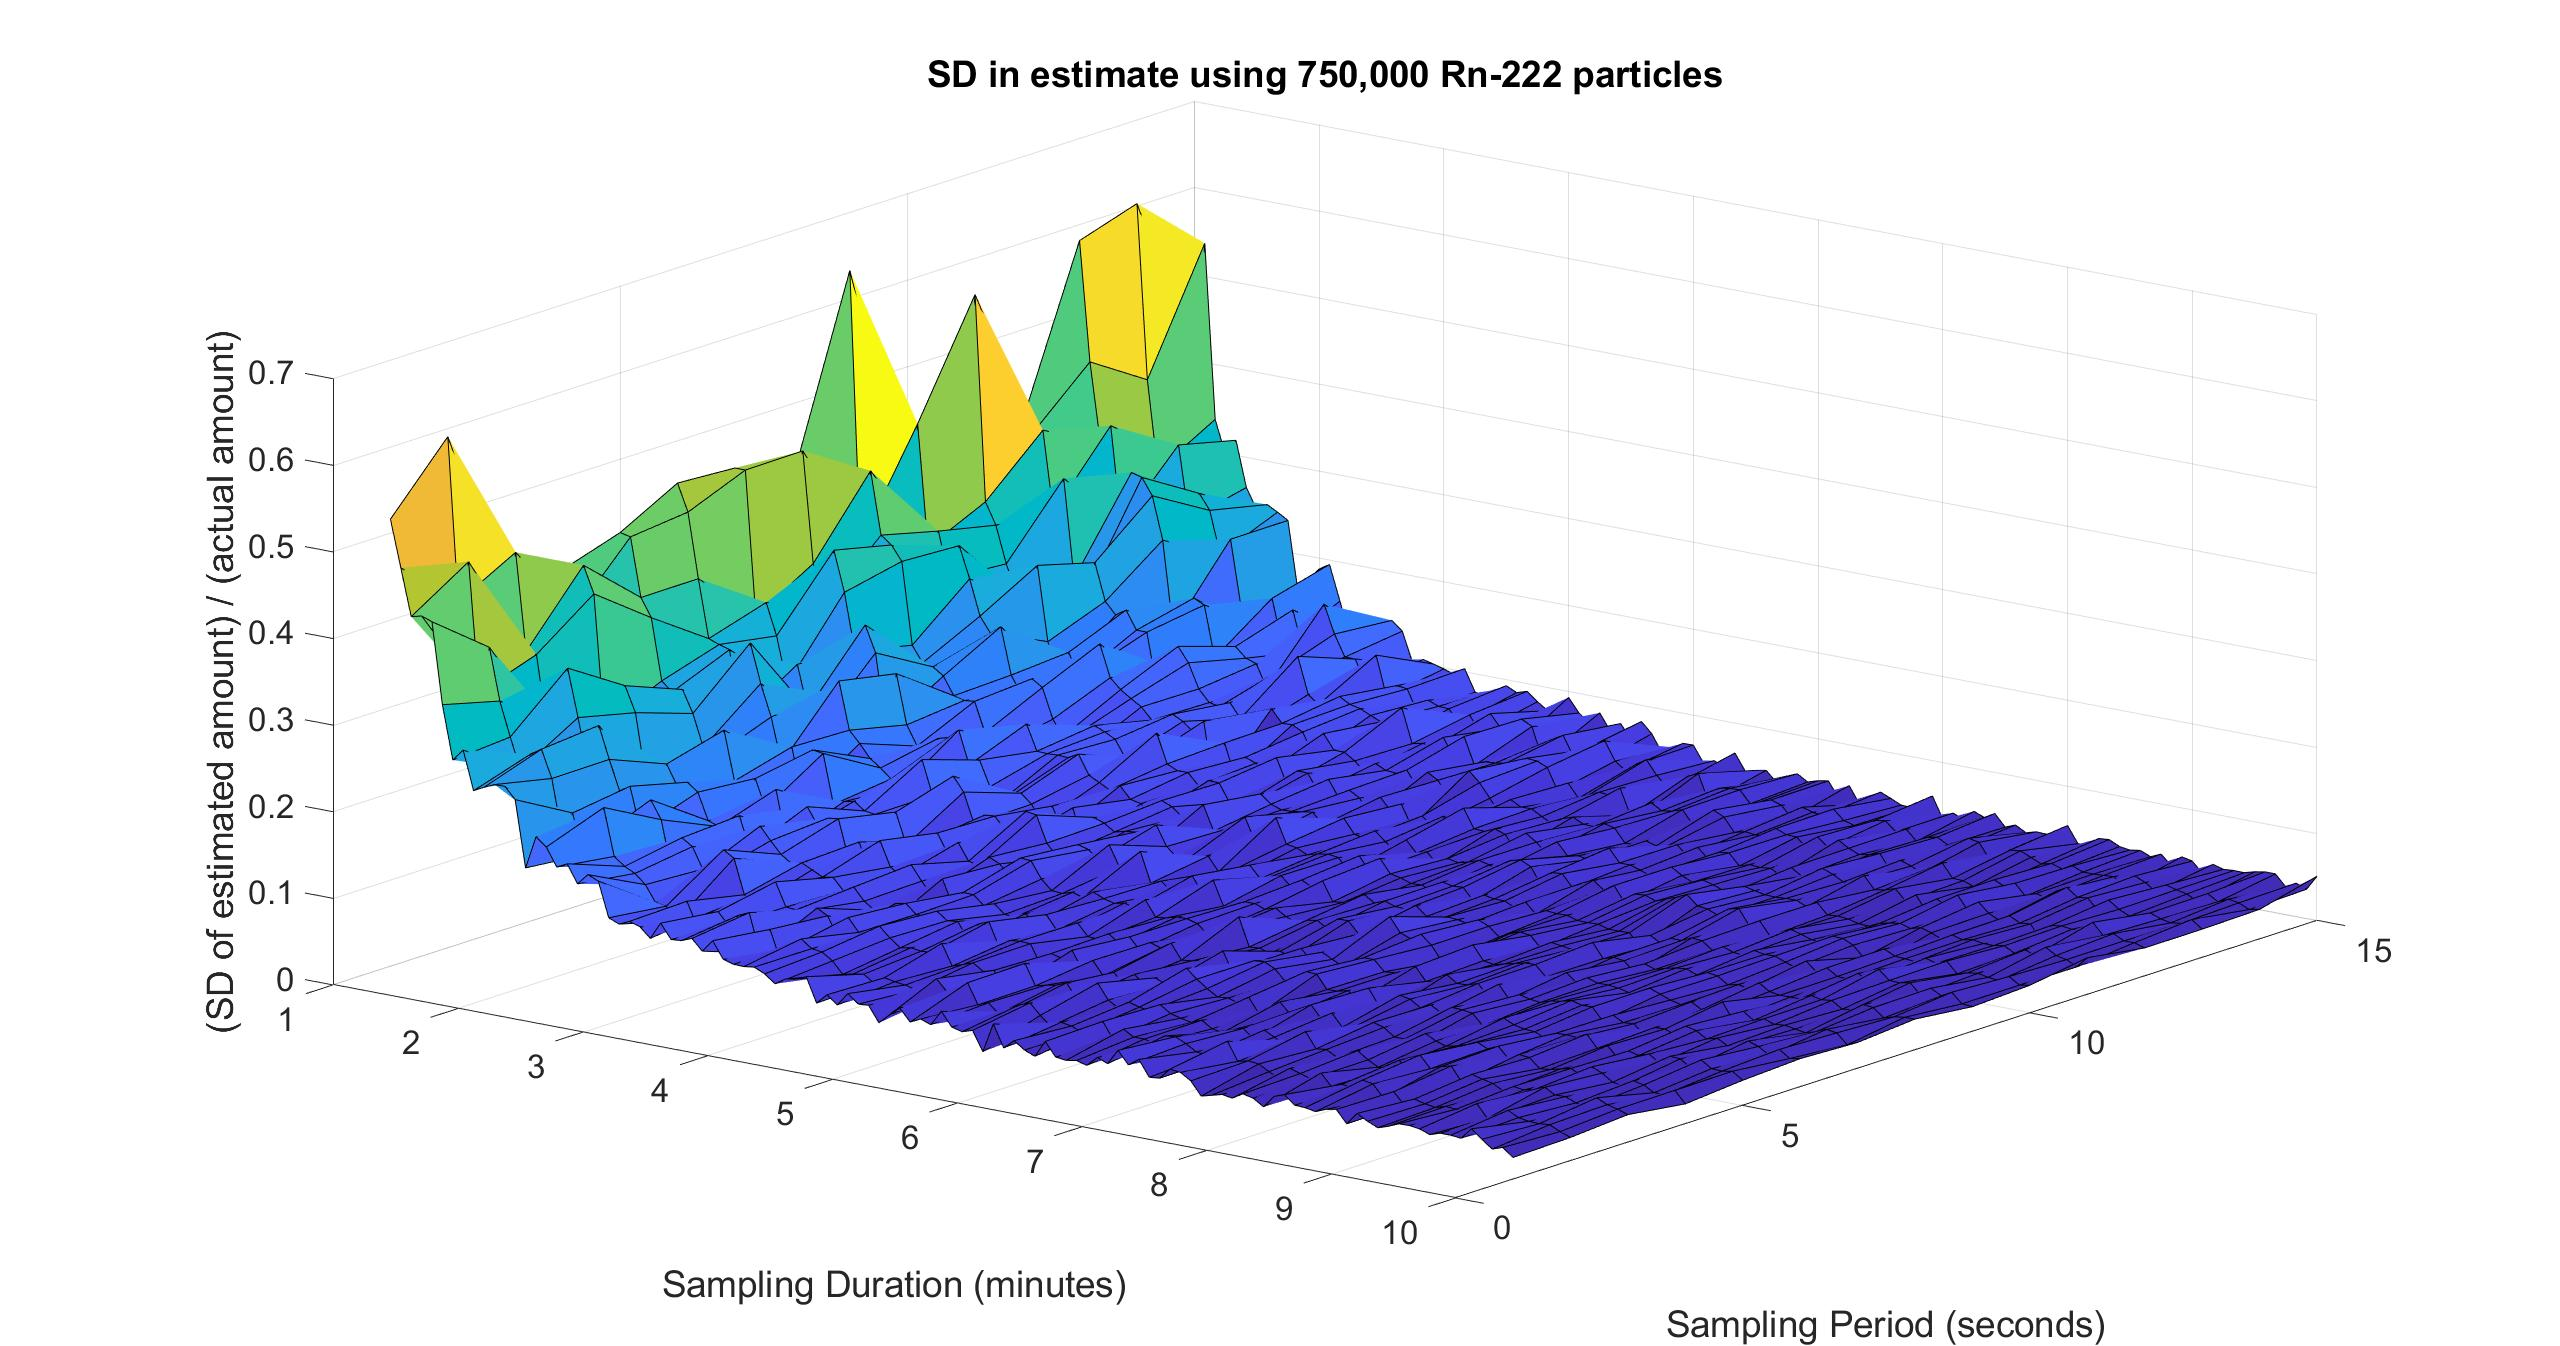
\includegraphics[width=\textwidth]{images/std_rn222_gridsearch.jpg}
\end{frame}

\begin{frame}{Grid Search}
    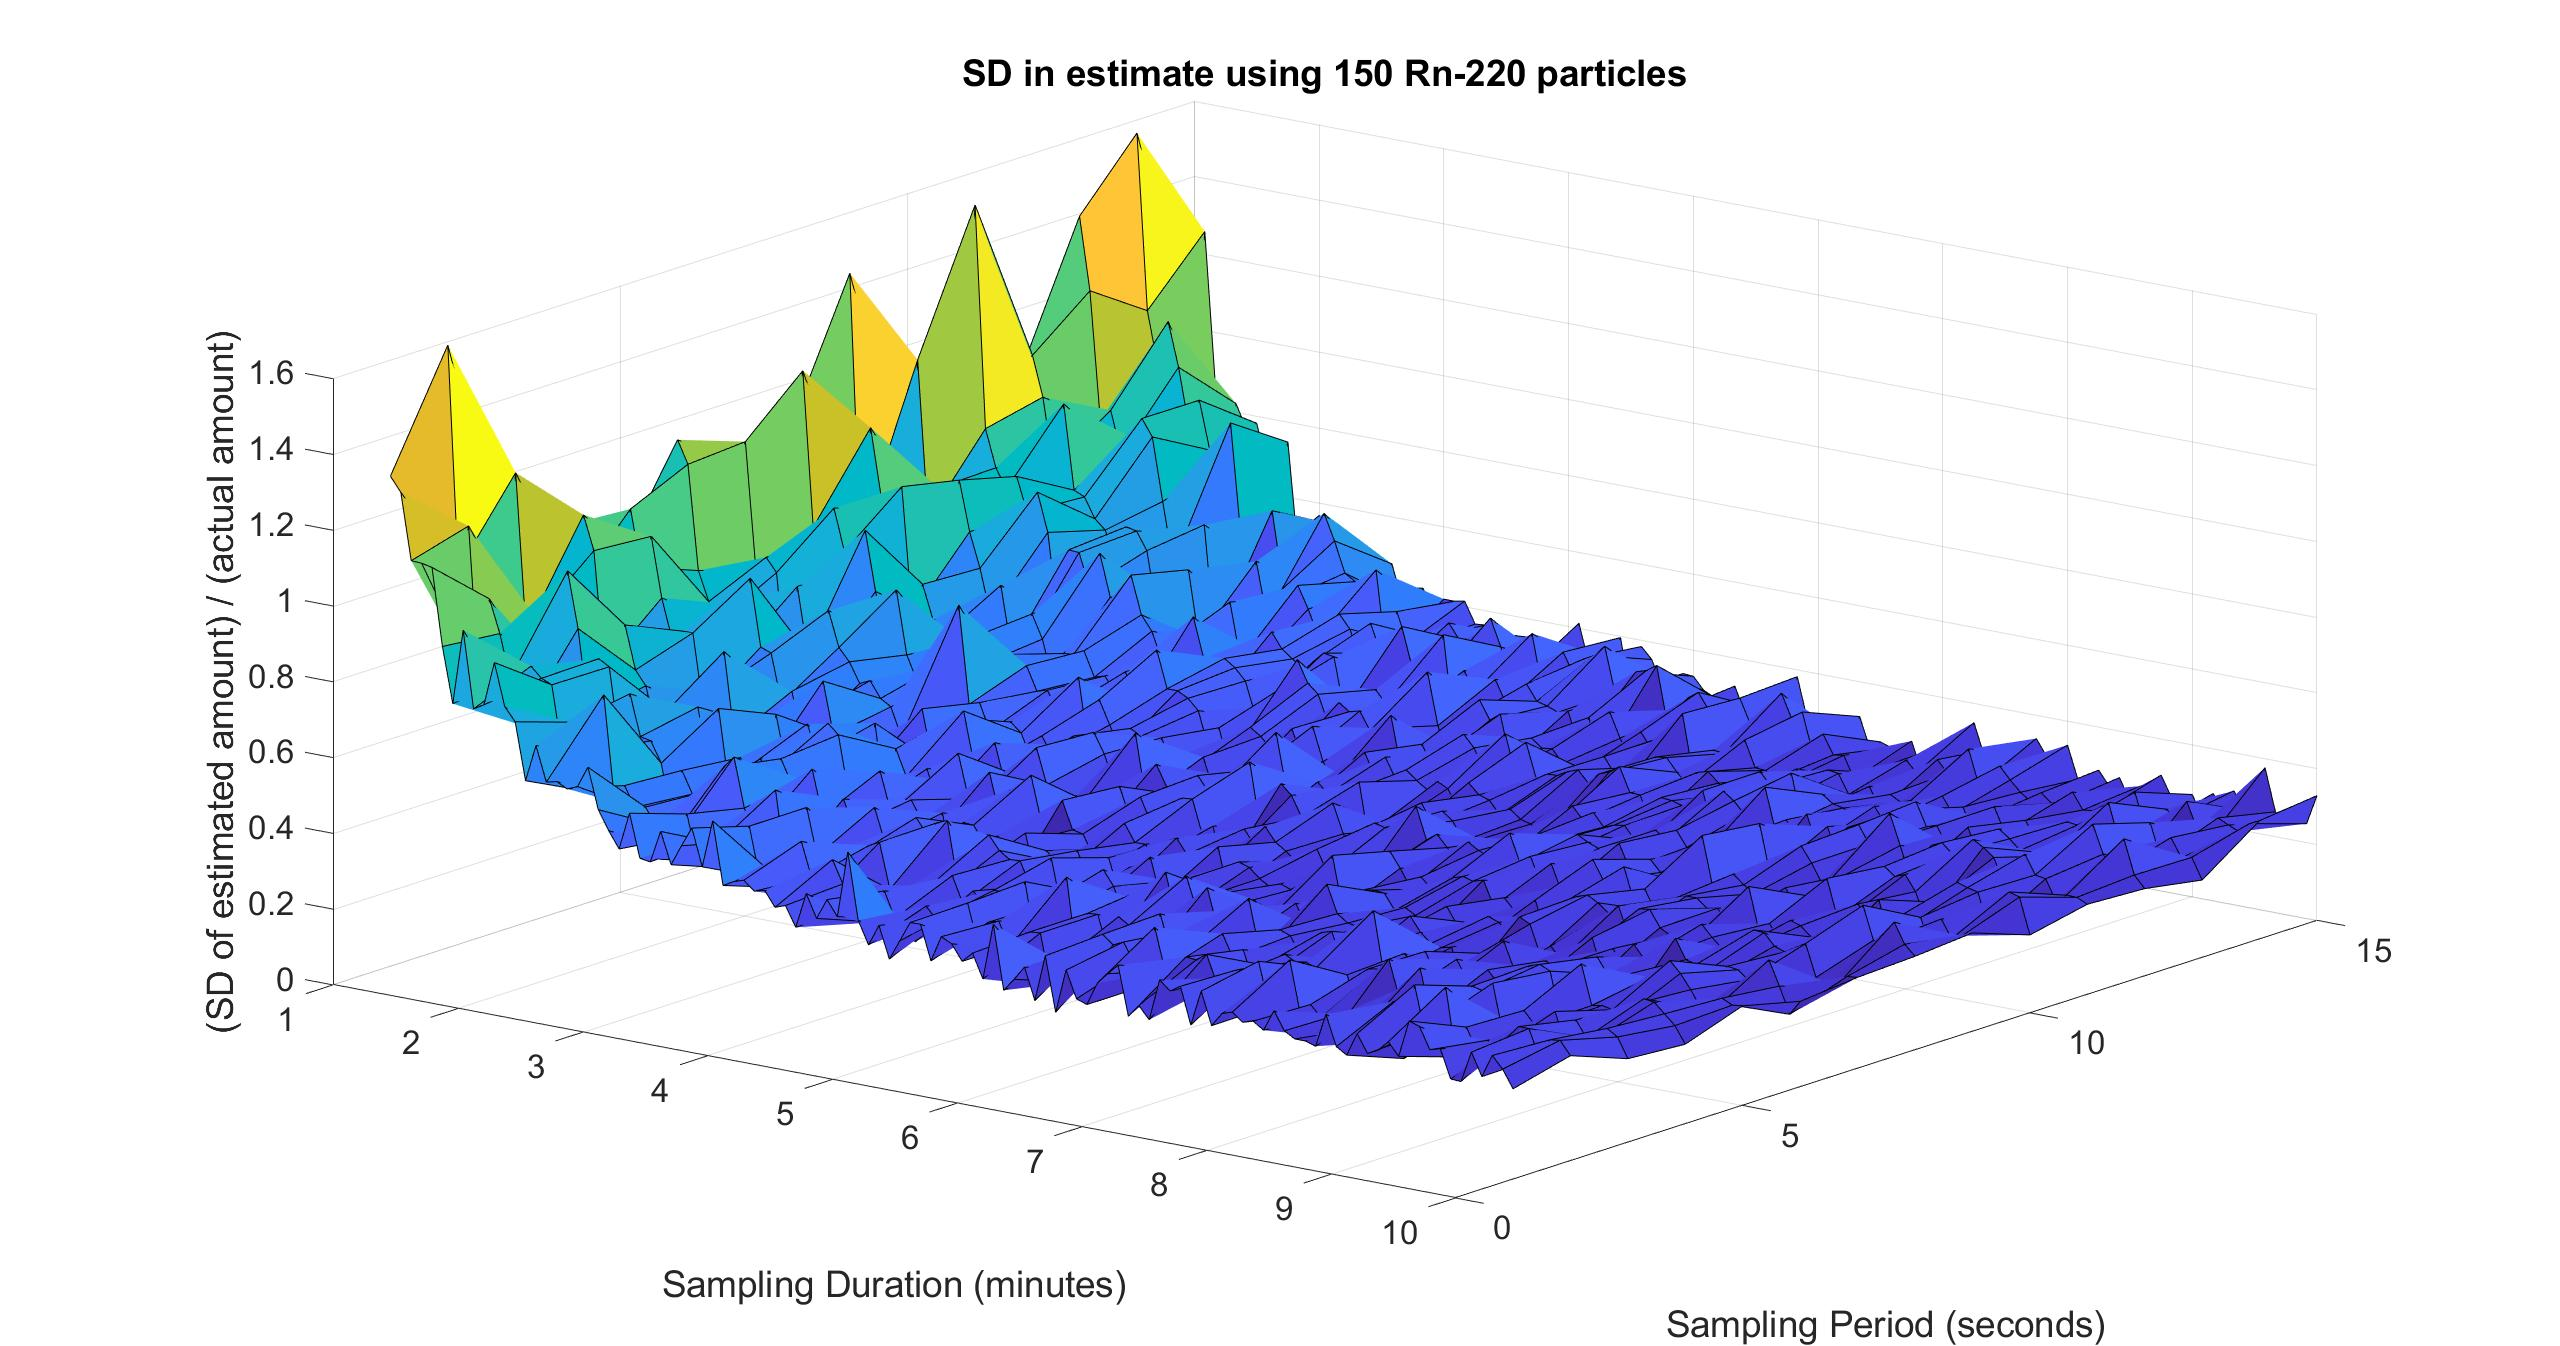
\includegraphics[width=\textwidth]{images/std_rn220_gridsearch.jpg}
\end{frame}

\subsection{Data Fitting}
{\nologo
\begin{frame}{Data Fitting - Radon Trial 1}
    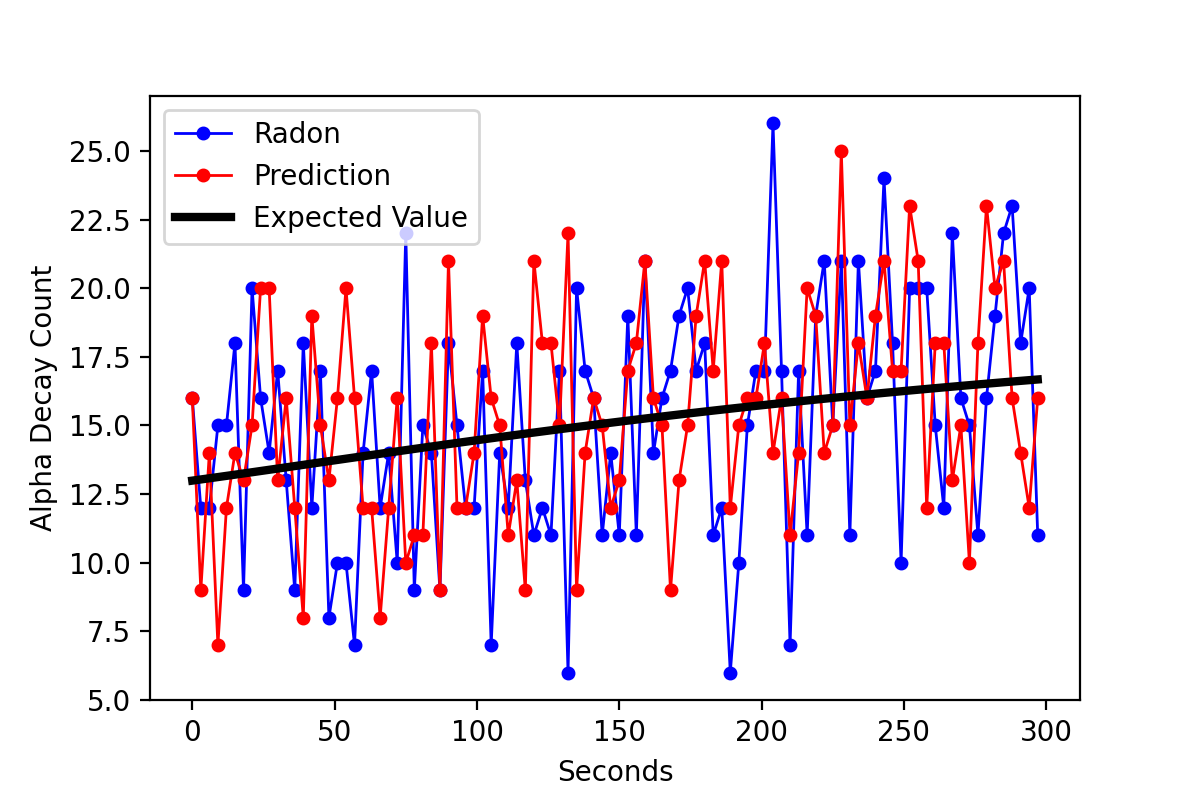
\includegraphics[width=\textwidth]{images/Radon_Trial1.png}
\end{frame}
\begin{frame}{Data Fitting - Radon Trial 2}
    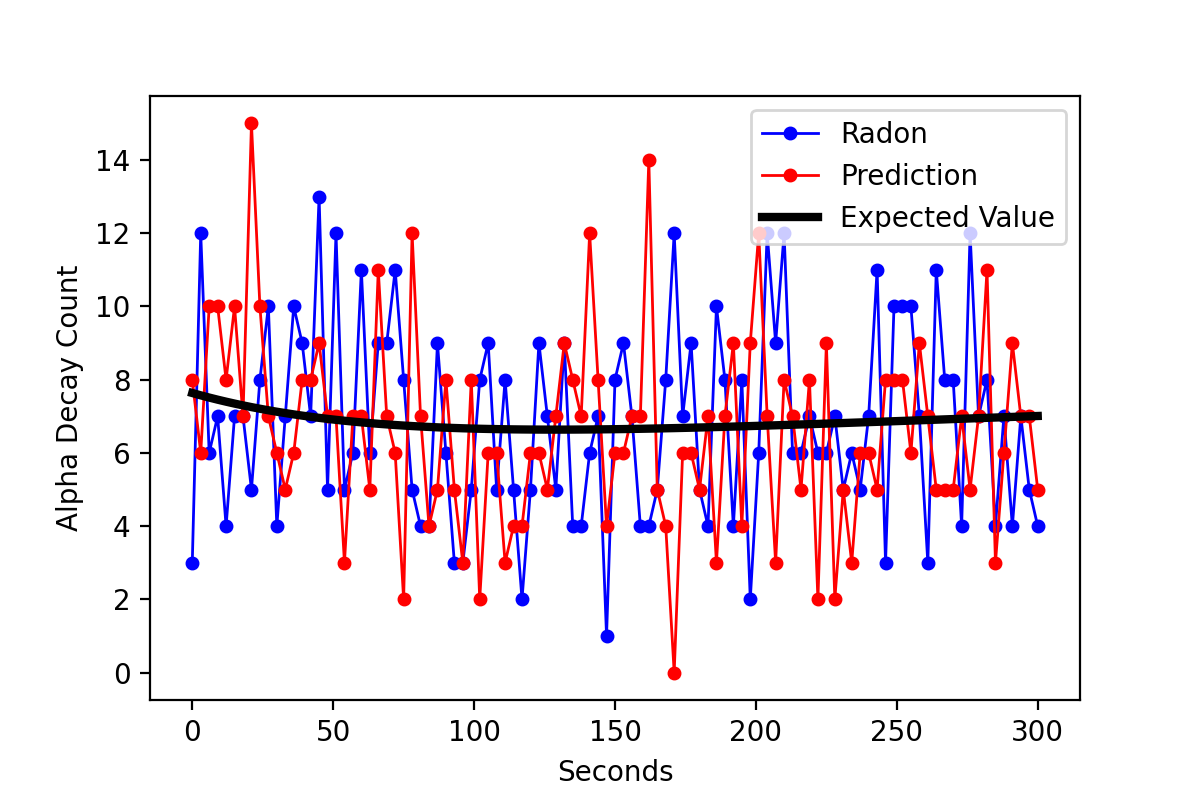
\includegraphics[width=\textwidth]{images/Radon_Trial2.png}
\end{frame}
\begin{frame}{Data Fitting - Radon Trial 3}
    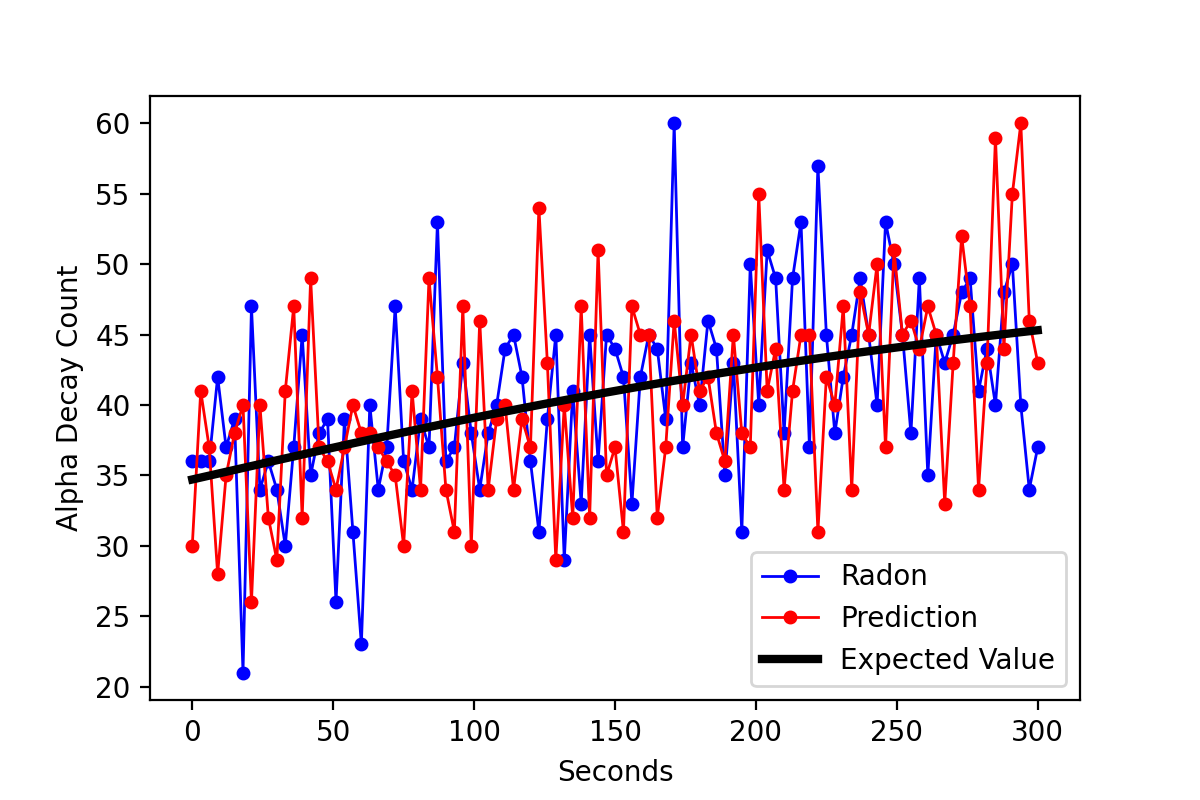
\includegraphics[width=\textwidth]{images/Radon_Trial3.png}
\end{frame}
\begin{frame}{Data Fitting - Thoron Trial}
    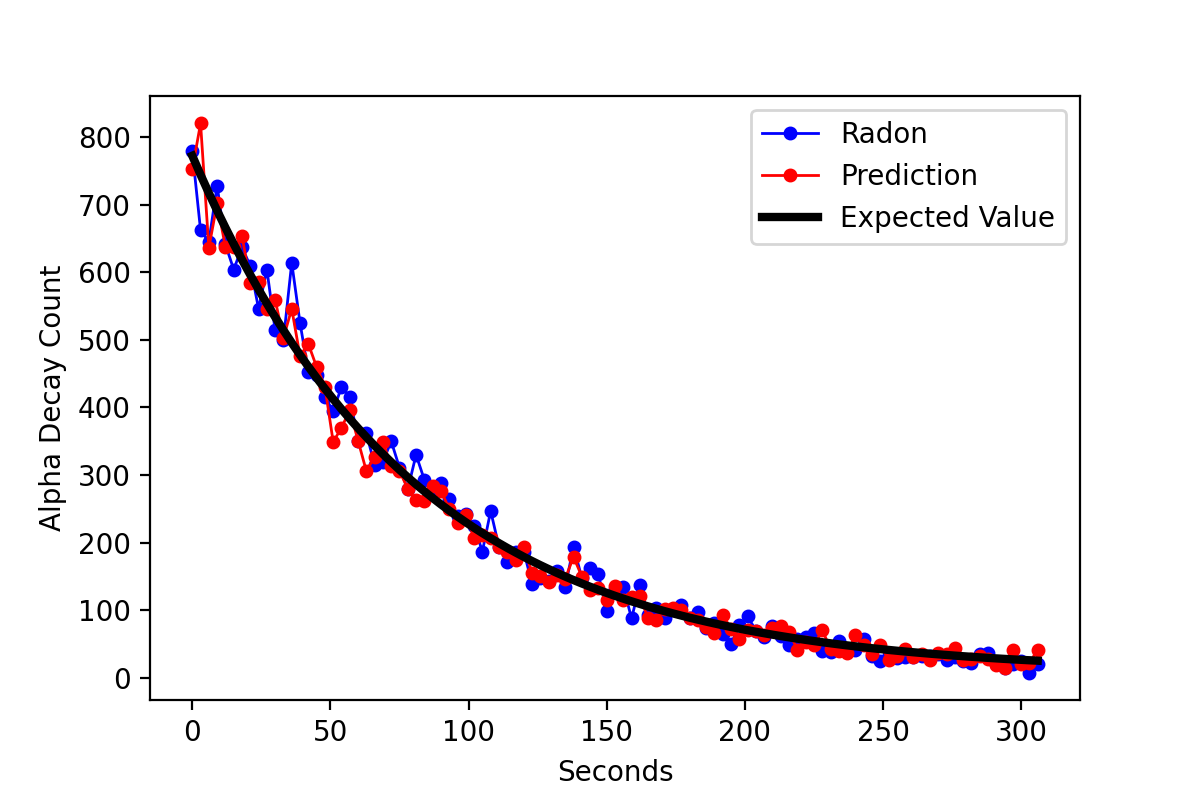
\includegraphics[width=\textwidth]{images/Thoron_Trial1.png}
\end{frame}
}
\section{Conclusion}
\begin{frame}{Conclusion}
    We would like to thank:
    \begin{itemize}
        \item PIMS for running this workshop and providing us with this opportunity
        \item Kai \& EIC, for letting us work on this problem and helping us through it
        \item The $\textit{Math}^{\textit{Industry}}$ organizers for all their work in setting up this workshop
        \item You, for listening to our presentation
    \end{itemize}
\end{frame}
\end{document}


% Data generation
% Model, sampling times and graphs 
% AR(1) model not working (maybe don't even talk about)
